% Define metadata
\documentclass{template/thesis}
\usepackage{subcaption}
\usepackage{graphicx}
\usepackage{float}
% --- Tinh chỉnh khoảng cách ---
% Khoảng cách giữa hình và văn bản
\setlength{\textfloatsep}{10pt plus 2pt minus 2pt}
\setlength{\intextsep}{10pt plus 2pt minus 2pt}
% Khoảng cách giữa 2 hình liên tiếp
\setlength{\floatsep}{10pt plus 2pt minus 2pt}
\Title{Tìm hiểu các thuật toán tổng hợp trọng số trong Federated Learning}
\Title[en]{A Study on Weight Aggregation Algorithms in Federated Learning}

\ThesisType{BÁO CÁO ĐỒ ÁN}

\University{ĐẠI HỌC QUỐC GIA THÀNH PHỐ HỒ CHÍ MINH}
\CollegeOrDept{{TRƯỜNG ĐẠI HỌC CÔNG NGHỆ THÔNG TIN}}
\Faculty{KHOA KHOA HỌC VÀ KỸ THUẬT THÔNG TIN}


\Author{PHẠM QUỐC CƯỜNG}{250201004}
\Author{LÊ QUANG MINH}{250201016}
\Author{NGUYỄN ĐĂNG PHÚC LỢI}{250202012}

\Degree{MÔN: AN TOÀN BẢO MẬT HỆ THỐNG THÔNG TIN}
% \MajorCode{123}
\ThesisYear{2025}
\ThesisLocation{TP. HỒ CHÍ MINH}

\Supervisor{PGS TS. Nguyễn Tấn Cầm}

\hypersetup{
	pdfencoding=auto,
	pdfauthor={Tên tác giả},
	pdfsubject={Chủ đề đề tài},
	pdftitle={Tên tiêu đề đề tài},
	pdfkeywords={}
}

\begin{document}
\firstbeforepreface
\secondbeforepreface
\setcounter{page}{1}
\newpage
\afterpreface

% Thông tin thành viên nhóm
\chapter*{Thông tin thành viên nhóm}
\addcontentsline{toc}{chapter}{Thông tin thành viên nhóm}

\vspace{1cm}

% Thành viên 1
\noindent
\begin{minipage}[t]{0.25\textwidth}
    \vspace{0pt}
    \centering
    
\includegraphics[width=0.9\textwidth]{img/member1.jpg}
\end{minipage}
\hfill
\begin{minipage}[t]{0.7\textwidth}
    \vspace{0pt}
    \textbf{\Large PHẠM QUỐC CƯỜNG}
    
    \vspace{0.3cm}
    
    \textbf{MSHV:} 250201004
    
    \textbf{Email:} cuongpq.20@grad.uit.edu.vn
    
\end{minipage}%

\vspace{1.5cm}

% Thành viên 2
\noindent
\begin{minipage}[t]{0.25\textwidth}
    \vspace{0pt}
    \centering
    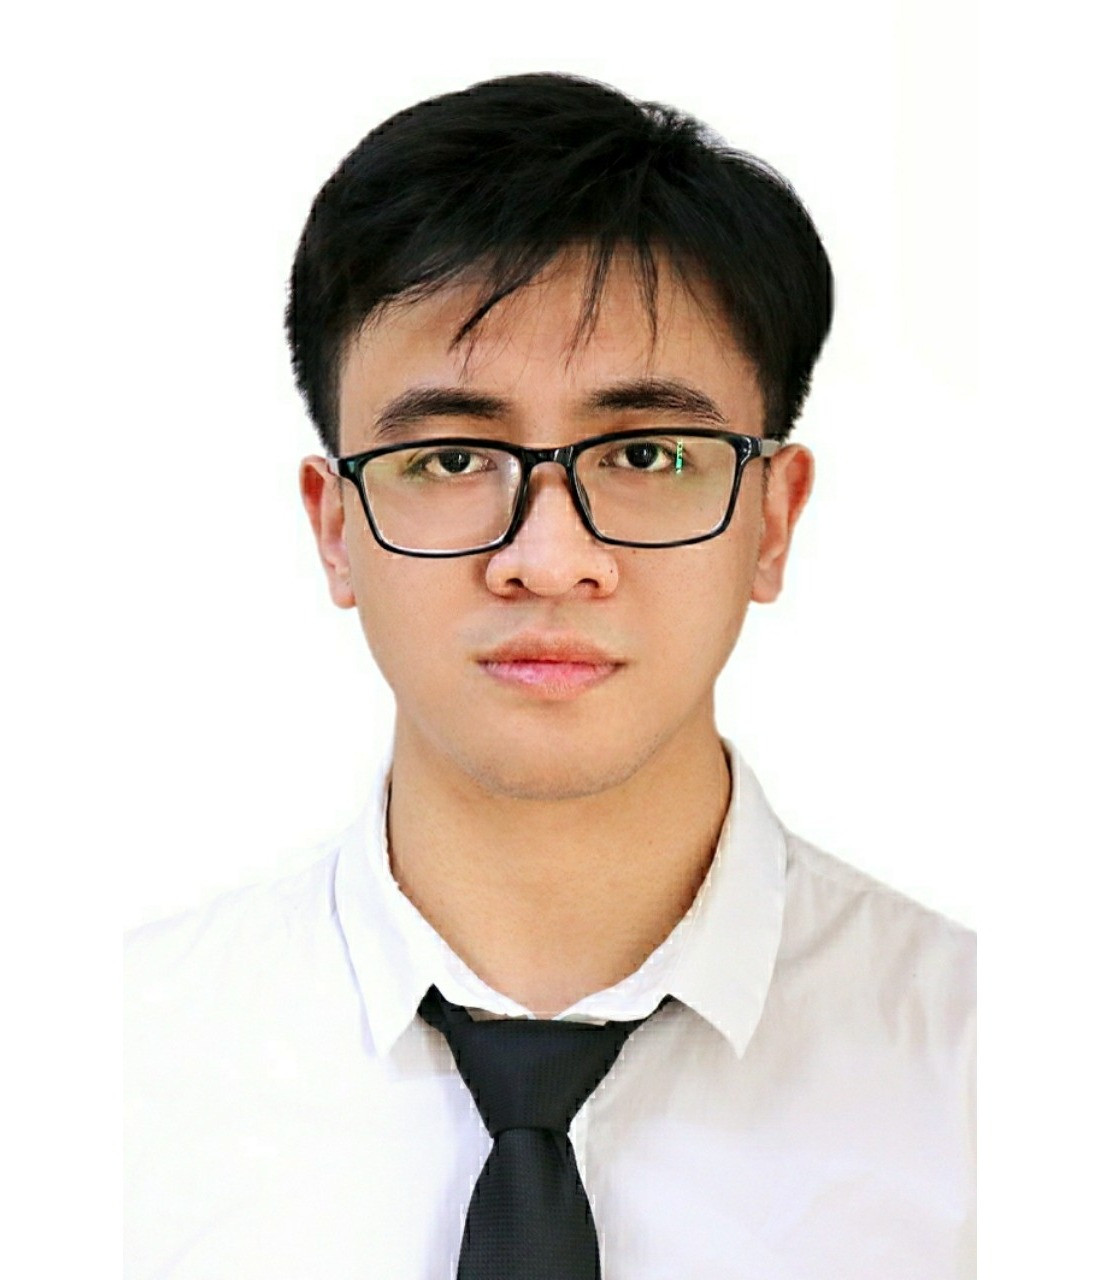
\includegraphics[width=0.9\textwidth]{img/member2.jpg}
\end{minipage}
\hfill
\begin{minipage}[t]{0.7\textwidth}
    \vspace{0pt}
    \textbf{\Large LÊ QUANG MINH}
    
    \vspace{0.3cm}
    
    \textbf{MSHV:} 250201016
    
    \textbf{Email:} minhlq.20@grad.uit.edu.vn
    
\end{minipage}%

\vspace{1.5cm}

% Thành viên 3
\noindent
\begin{minipage}[t]{0.25\textwidth}
    \vspace{0pt}
    \centering
    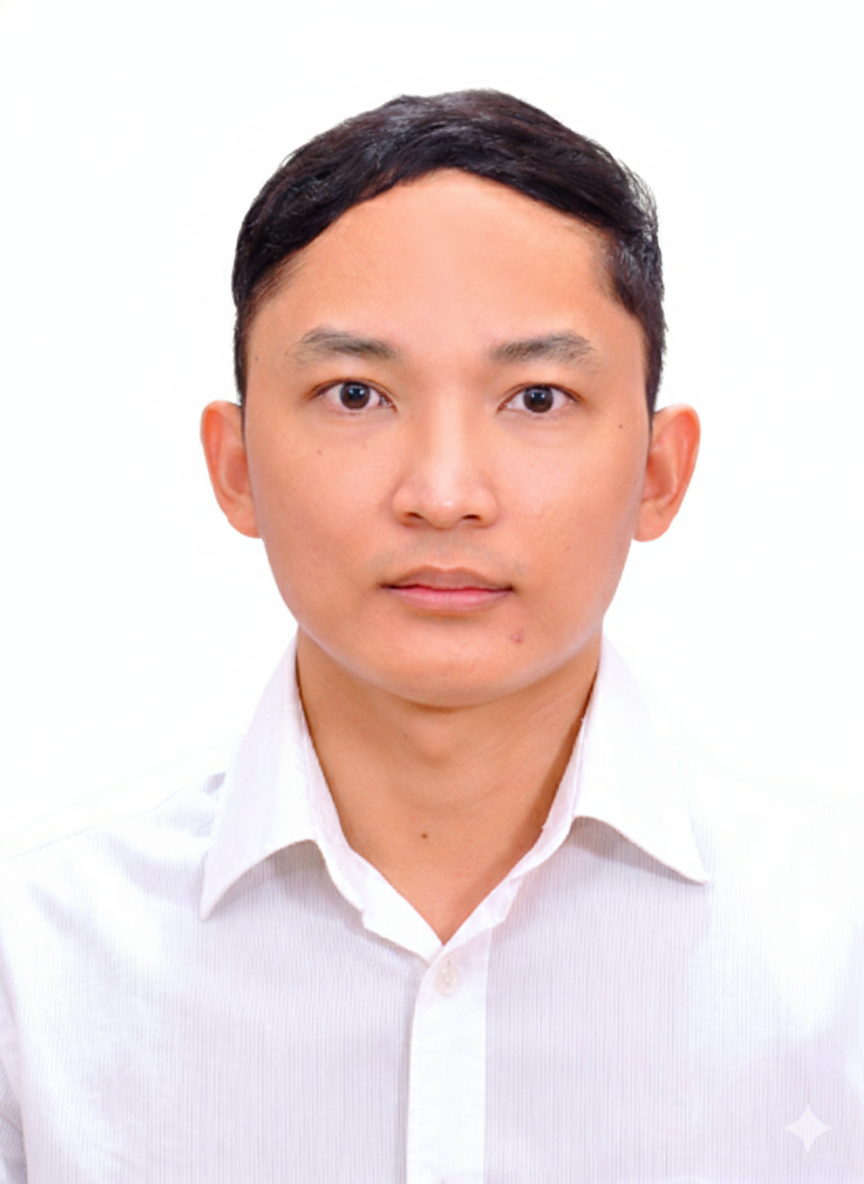
\includegraphics[width=0.9\textwidth]{img/member3.jpg}
\end{minipage}
\hfill
\begin{minipage}[t]{0.7\textwidth}
    \vspace{0pt}
    \textbf{\Large NGUYỄN ĐĂNG PHÚC LỢI}
    
    \vspace{0.3cm}
    
    \textbf{MSHV:} 250202012
    
    \textbf{Email:} loindp.20@grad.uit.edu.vn
    
\end{minipage}%

\vspace{2cm}


\clearpage

\chapter{Mở đầu}
\label{c:intro}
\section{Lý do chọn đề tài}
Trong kỷ nguyên của cuộc Cách mạng Công nghiệp 4.0, Trí tuệ nhân tạo \ac{ai} và Học máy \ac{ml} đã trở thành những công cụ không thể thiếu, thúc đẩy sự phát triển vượt bậc trong các lĩnh vực như y tế thông minh, tài chính số và xe tự lái, ... Tuy nhiên, các mô hình học máy truyền thống thường dựa trên kiến trúc tập trung, đòi hỏi dữ liệu từ nhiều nguồn phải được thu thập và lưu trữ tại một máy chủ duy nhất để huấn luyện. Cách tiếp cận này đang đối mặt với "rào cản dữ liệu" cực kỳ lớn khi các quy định về quyền riêng tư ngày càng siết chặt. Sự ra đời của các khung pháp lý như Quy định bảo vệ dữ liệu chung (GDPR) của Liên minh Châu Âu \cite{Voigt2017} hay Đạo luật quyền riêng tư của người tiêu dùng California (CCPA) đã khiến việc chia sẻ dữ liệu thô trở thành một rủi ro pháp lý và đạo đức nghiêm trọng \cite{Zhang2021Survey}.

Federated Learning \ac{fl} (Học tập liên hợp) xuất hiện như một lời giải cho bài toán "ốc đảo dữ liệu" (Data Silos), cho phép các thiết bị biên cộng tác huấn luyện mô hình mà không cần truyền tải dữ liệu gốc \cite{McMahan2017}. Mặc dù \ac{fl} mang lại lợi thế vượt trội về bảo mật, việc triển khai nó trong môi trường thực tế vấp phải thách thức cốt lõi là sự không đồng nhất về dữ liệu (Non-IID).[1][2] Trong kịch bản này, dữ liệu giữa các người dùng thường bị lệch về phân phối nhãn (Label Skew) hoặc đặc trưng (Feature Skew), gây ra hiện tượng "trôi dạt trọng số" (Weight Drift) \cite{Zhao2018}. Các thuật toán cơ bản như FedAvg thường mất đi tính ổn định và khó hội tụ khi đối mặt với sự phân hóa dữ liệu cực đoan này \cite{Li2020}.

Trước những hạn chế đó, giai đoạn 2022-2025 chứng kiến sự bùng nổ của các chiến lược tổng hợp trọng số tiên tiến nhằm tối ưu hóa hiệu năng và tính bền vững của hệ thống. Các nghiên cứu đột phá như FedLWS \cite{Shi2025LWS} đã đề xuất cơ chế co trọng số theo từng lớp để xử lý sự khác biệt về độ sâu mạng nơ-ron, trong khi FedAWA \cite{Shi2025AWA} sử dụng các vector client để điều chỉnh trọng số thích ứng, giúp mô hình bám sát hướng tối ưu toàn cầu. Bên cạnh đó, các phương pháp như FedNolowe \cite{Le2025} tập trung vào việc chuẩn hóa hàm loss để giảm thiểu tác động của các client có dữ liệu nhiễu, và FedProto \cite{Tan2022} thay thế việc truyền tải tham số bằng các đại diện lớp (prototypes) để vượt qua rào cản về kiến trúc mô hình không đồng nhất.

Tuy nhiên, dù có nhiều cải tiến, việc lựa chọn thuật toán nào phù hợp cho từng ngữ cảnh cụ thể — giữa sự đánh đổi về độ chính xác, chi phí truyền thông và khả năng chống lại các cuộc tấn công đầu độc mô hình \cite{Fang2020} — vẫn là một câu hỏi mở. Đặc biệt, sự thiếu hụt các nghiên cứu đối chứng toàn diện giữa các thuật toán SOTA (State-of-the-art) mới nhất khiến các nhà phát triển gặp khó khăn trong việc triển khai thực tế. Đồng thời, nhu cầu về một phương pháp vừa đảm bảo hiệu năng trong môi trường Non-IID, vừa tăng cường tính an toàn (Security) là vô cùng cấp thiết.

Xuất phát từ những bối cảnh trên, đề tài "Tìm hiểu các thuật toán tổng hợp trọng số trong Federated Learning" được thực hiện nhằm phân tích sâu sắc cơ chế toán học, so sánh hiệu năng thực nghiệm và đánh giá tính khả thi của các thuật toán hàng đầu hiện nay. Đề tài không chỉ dừng lại ở việc khảo sát mà còn hướng tới việc đề xuất giải pháp FedSecL, nhằm thu hẹp khoảng cách giữa hiệu năng huấn luyện và tính an toàn dữ liệu trong các hệ thống \ac{fl} thế hệ mới.

\section{Các nghiên cứu liên quan}
Các nghiên cứu trong lĩnh vực \ac{fl} đã trải qua nhiều giai đoạn phát triển để giải quyết các vấn đề về phân phối dữ liệu và tính thích nghi:

\begin{itemize}
  \item \textbf{FedAvg:} Thuật toán cơ bản nhất sử dụng trung bình trọng số dựa trên kích thước dữ liệu\cite{McMahan2017}. Tuy nhiên, hiệu suất giảm mạnh khi dữ liệu Non-IID.
  \item \textbf{FedLWS:} Đề xuất phương pháp co trọng số theo từng lớp (layer-wise weight shrinking) để tối ưu hóa quá trình tổng hợp mà không cần dữ liệu proxy\cite{Shi2025LWS}.
  \item \textbf{FedAWA:} Sử dụng "client vector" để điều chỉnh trọng số thích ứng, gán trọng số cao hơn cho các cập nhật phù hợp với hướng tối ưu toàn cầu\cite{Shi2025AWA}.
  \item \textbf{FedNolowe:} Sử dụng giá trị loss đã được chuẩn hóa hai giai đoạn để tính toán trọng số, giúp mô hình ổn định hơn trước dữ liệu nhiễu\cite{Le2025}.
  \item \textbf{FedProto:} Truyền tải các prototype (đại diện lớp) thay vì tham số mô hình, giúp giải quyết vấn đề không đồng nhất về kiến trúc mô hình\cite{Tan2022}.

\end{itemize}

\section{Mục tiêu, đối tượng và phạm vi nghiên cứu}

\subsection{Mục tiêu nghiên cứu}
\label{sec:MucTieu}
Mục tiêu của đề tài là tìm hiểu, phân tích và so sánh hiệu quả của các chiến lược học tập tiên tiến trong \ac{fl}. Cụ thể:
\begin{itemize}
    \item Phân tích cơ chế toán học của các thuật toán tổng hợp trọng số tiên tiến: FedAvg, FedLWS, FedAWA, FedNolowe, FedProto.
    \item So sánh hiệu suất của các thuật toán trên dữ liệu IID và Non-IID.
    \item Đánh giá khả năng hội tụ, độ chính xác và chi phí tính toán của từng thuật toán.
\end{itemize}

\subsection{Đối tượng nghiên cứu}
\label{sec:DoiTuong}
Đối tượng nghiên cứu bao gồm:
\begin{itemize}
    \item Các thuật toán tổng hợp mô hình (Aggregation Algorithms): FedAvg, FedLWS, FedAWA, FedNolowe, và FedProto.
    \item Các mô hình mạng nơ-ron tích chập (CNN, ResNet) trong bài toán phân loại ảnh.
\end{itemize}

\subsection{Phạm vi nghiên cứu}
\label{sec:PhamVi}
Đề tài thực hiện khảo sát và đánh giá trong phạm vi:
\begin{itemize}
    \item Dữ liệu: MNIST và CIFAR-10 với thiết lập phân phối IID và Non-IID.
    \item Môi trường: Giả lập hệ thống \ac{fl} với nhiều client tham gia huấn luyện đồng thời.
\end{itemize}

\section{Phương pháp nghiên cứu}
\label{sec:PhuongPhap}
Đề tài áp dụng các phương pháp nghiên cứu sau:
\begin{enumerate}
    \item \textbf{Nghiên cứu tài liệu:} Tổng hợp và phân tích các bài báo khoa học (SOTA) từ năm 2022 đến 2025 về các thuật toán tổng hợp trọng số trong \ac{fl}.
    \item \textbf{Phân tích so sánh:} Đối chiếu các đặc điểm kỹ thuật như độ phức tạp tính toán, thời gian huấn luyện và hiệu suất trên dữ liệu Non-IID.
    \item \textbf{Tổng hợp kết quả:} Dựa trên kết quả thực nghiệm từ các công bố gốc để so sánh hiệu năng (Accuracy, Convergence Speed) giữa các phương pháp.
\end{enumerate}

\section{Các đóng góp chính của đề tài}
\label{sec:DongGop}
Báo cáo này mang lại các đóng góp chính:
\begin{itemize}
    \item Cung cấp cái nhìn toàn diện về các kỹ thuật tổng hợp trọng số tiên tiến (2022-2025) như FedLWS, FedAWA, FedNolowe và FedProto.
    \item Phân tích chi tiết hiệu suất của các thuật toán trên dữ liệu IID và Non-IID thông qua các thí nghiệm trên bộ dữ liệu MNIST và CIFAR-10.
    \item Đề xuất một phương pháp để giải quyết "khoảng trống" của các phương pháp đã có.
    \item Đề xuất bảng so sánh tổng hợp về accuracy, thời gian huấn luyện và độ phức tạp giúp lựa chọn thuật toán phù hợp cho từng ngữ cảnh triển khai.
\end{itemize}

\section{Cấu trúc Báo cáo đề tài}
\label{sec:CauTruc}
Báo cáo với tên đề tài ``Tìm hiểu các thuật toán tổng hợp trọng số trong Federated Learning'' được trình bày bao gồm 5 chương:
\begin{itemize}
    \item \textbf{Chương 1: Mở đầu.} Giới thiệu tổng quan về bối cảnh, lý do chọn đề tài và mục tiêu nghiên cứu.
    \item \textbf{Chương 2: Cơ sở lý thuyết.} Trình bày các kiến thức nền tảng về \ac{fl} và phân tích chi tiết 5 thuật toán: FedAvg, FedLWS, FedAWA, FedNolowe, FedProto.
    \item \textbf{Chương 3: Phương pháp đề xuất: FedSecL.} Trình bày phương pháp nghiên cứu đề xuất
    \item \textbf{Chương 4: Phương pháp thực hiện.} Trình bày phương pháp nghiên cứu, tiêu chí so sánh và môi trường thực nghiệm.
    \item \textbf{Chương 5: Đánh giá và thảo luận.} So sánh kết quả thực nghiệm và phân tích hiệu quả của từng phương pháp.
    \item \textbf{Chương 6: Tổng kết.} Tóm tắt kết quả đạt được và định hướng phát triển.
\end{itemize}

\chapter{Cơ sở lý thuyết}
\label{c:cosolythuyet}
Chương này trình bày các khái niệm nền tảng về Federated Learning và đi sâu phân tích cơ sở toán học của các thuật toán tổng hợp trọng số. Phần đầu sẽ giới thiệu thuật toán kinh điển FedAvg, đóng vai trò là mốc cơ sở (baseline). Phần tiếp theo sẽ phân tích thuật toán tiên tiến FedLWS, một phương pháp mới được đề xuất năm 2025 giúp cải thiện khả năng tổng quát hóa thông qua cơ chế co trọng số thích ứng.

\section{Tổng quan về Federated Learning}
Học máy liên kết (\ac{fl}) là một mô hình huấn luyện máy học phi tập trung, cho phép nhiều thiết bị (clients) cộng tác để học một mô hình chia sẻ toàn cầu mà vẫn giữ dữ liệu huấn luyện nằm cục bộ trên thiết bị \cite{McMahan2017}. Mục tiêu của \ac{fl} là tối ưu hóa hàm mục tiêu có dạng tổng hữu hạn:
\begin{equation}
    \min_{w \in \mathbb{R}^d} f(w) \quad \text{với} \quad f(w) \stackrel{\text{def}}{=} \frac{1}{n} \sum_{i=1}^{n} f_i(w)
\end{equation}
Trong đó, $f_i(w) = \ell(x_i, y_i; w)$ là hàm mất mát (loss function) trên mẫu dữ liệu $(x_i, y_i)$ với tham số mô hình $w$ \cite{McMahan2017}.


\section{Thuật toán Federated Averaging (FedAvg)}
\label{sec:FedAvg}

\subsection{Tổng quan và Cơ sở lý thuyết}
\textbf{Federated Averaging (FedAvg)}, được đề xuất bởi McMahan và cộng sự vào năm 2017, là thuật toán tối ưu hóa nền tảng cho Học máy liên kết (\ac{fl}) \cite{McMahan2017}. Thuật toán này ra đời nhằm giải quyết bài toán tối ưu hóa hàm mục tiêu toàn cầu $f(w)$ mà không cần truy cập trực tiếp vào dữ liệu thô nằm phân tán trên các thiết bị.

Về mặt toán học, mục tiêu của FedAvg là tìm tham số $w \in \mathbb{R}^d$ để tối thiểu hóa hàm mất mát tổng hợp:
\begin{equation}
    \min_{w} f(w) \quad \text{với} \quad f(w) \stackrel{\text{def}}{=} \sum_{k=1}^{K} \frac{n_k}{n} F_k(w)
\end{equation}
Trong đó:
\begin{itemize}
    \item $K$ là tổng số lượng client tham gia.
    \item $n_k$ là số lượng mẫu dữ liệu tại client $k$, và $n = \sum_{k} n_k$ là tổng dữ liệu toàn hệ thống.
    \item $F_k(w) = \frac{1}{n_k} \sum_{i \in \mathcal{P}_k} \ell(x_i, y_i; w)$ là hàm mất mát cục bộ (Local Loss Function) trên tập dữ liệu $\mathcal{P}_k$ của client $k$.
\end{itemize}

Động lực chính của FedAvg là khắc phục hạn chế về chi phí truyền thông của phương pháp tiền nhiệm \textit{FederatedSGD}. Thay vì đồng bộ hóa gradient sau mỗi bước tính toán đơn lẻ, FedAvg cho phép client thực hiện nhiều vòng lặp huấn luyện (epochs) để tính toán một cập nhật trọng số "chất lượng hơn" trước khi gửi đi, qua đó giảm thiểu số lần giao tiếp với máy chủ \cite{McMahan2017}.

\subsection{Quy trình hoạt động chi tiết}
Quá trình huấn luyện của FedAvg là một quy trình lặp (iterative process) gồm $T$ vòng giao tiếp (communication rounds). Tại mỗi vòng $t$, các bước thực hiện cụ thể như sau:

{Bước 1: Lựa chọn và Phân phối (Selection \& Broadcast)}
Tại đầu vòng $t$, máy chủ trung tâm (Server) chọn ngẫu nhiên một tập hợp con $S_t$ gồm $m$ client từ tổng số $K$ client khả dụng, với tỷ lệ tham gia $C$ ($m = \max(C \cdot K, 1)$). 
Máy chủ gửi tham số mô hình toàn cầu hiện tại $w_t$ đến tất cả các clients trong tập $S_t$.

{Bước 2: Tối ưu hóa cục bộ (Local Client Update)}
Mỗi client $k \in S_t$ nhận tham số $w_t$ và sao chép thành tham số cục bộ: $w_{t}^k \leftarrow w_t$.
Client thực hiện huấn luyện mô hình trên dữ liệu riêng $\mathcal{P}_k$ bằng thuật toán \textit{Stochastic Gradient Descent (SGD)}. Quá trình này diễn ra trong $E$ epochs (kỷ nguyên) với kích thước batch $B$ và tốc độ học $\eta$.

Quy tắc cập nhật cho mỗi bước lặp cục bộ (với batch dữ liệu $b \subset \mathcal{P}_k$):
\begin{equation}
    w^k \leftarrow w^k - \eta \nabla F_k(w^k; b)
\end{equation}
Sau khi hoàn thành $E$ epochs, client thu được bộ tham số đã cập nhật $w_{t+1}^k$.

\textit{Lưu ý:} Nếu $E=1$ và $B=n_k$ (full-batch), thuật toán trở về tương đương với FedSGD. Việc tăng $E > 1$ chính là chìa khóa giúp FedAvg hội tụ nhanh hơn về mặt truyền thông \cite{McMahan2017}.

{Bước 3: Tải lên tham số (Upload)}
Các client gửi vector tham số $w_{t+1}^k$ (hoặc vector chênh lệch $\Delta w^k = w_{t+1}^k - w_t$) trở lại máy chủ. Chỉ có trọng số mô hình được truyền đi, đảm bảo tính riêng tư dữ liệu.

{Bước 4: Tổng hợp trọng số (Aggregation)}
Máy chủ cập nhật mô hình toàn cầu bằng cách tính trung bình có trọng số (Weighted Averaging) các tham số nhận được. Trọng số quy định mức độ đóng góp của client dựa trên lượng dữ liệu sở hữu:
\begin{equation}
    w_{t+1} \leftarrow \sum_{k \in S_t} \frac{n_k}{n_{S_t}} w_{t+1}^k
\end{equation}
Trong đó $n_{S_t} = \sum_{k \in S_t} n_k$. Tham số $w_{t+1}$ được dùng làm đầu vào cho vòng $t+1$.

\begin{center}
    \begin{minipage}{\linewidth} % Dùng minipage để bó ảnh và caption lại với nhau
        \centering
        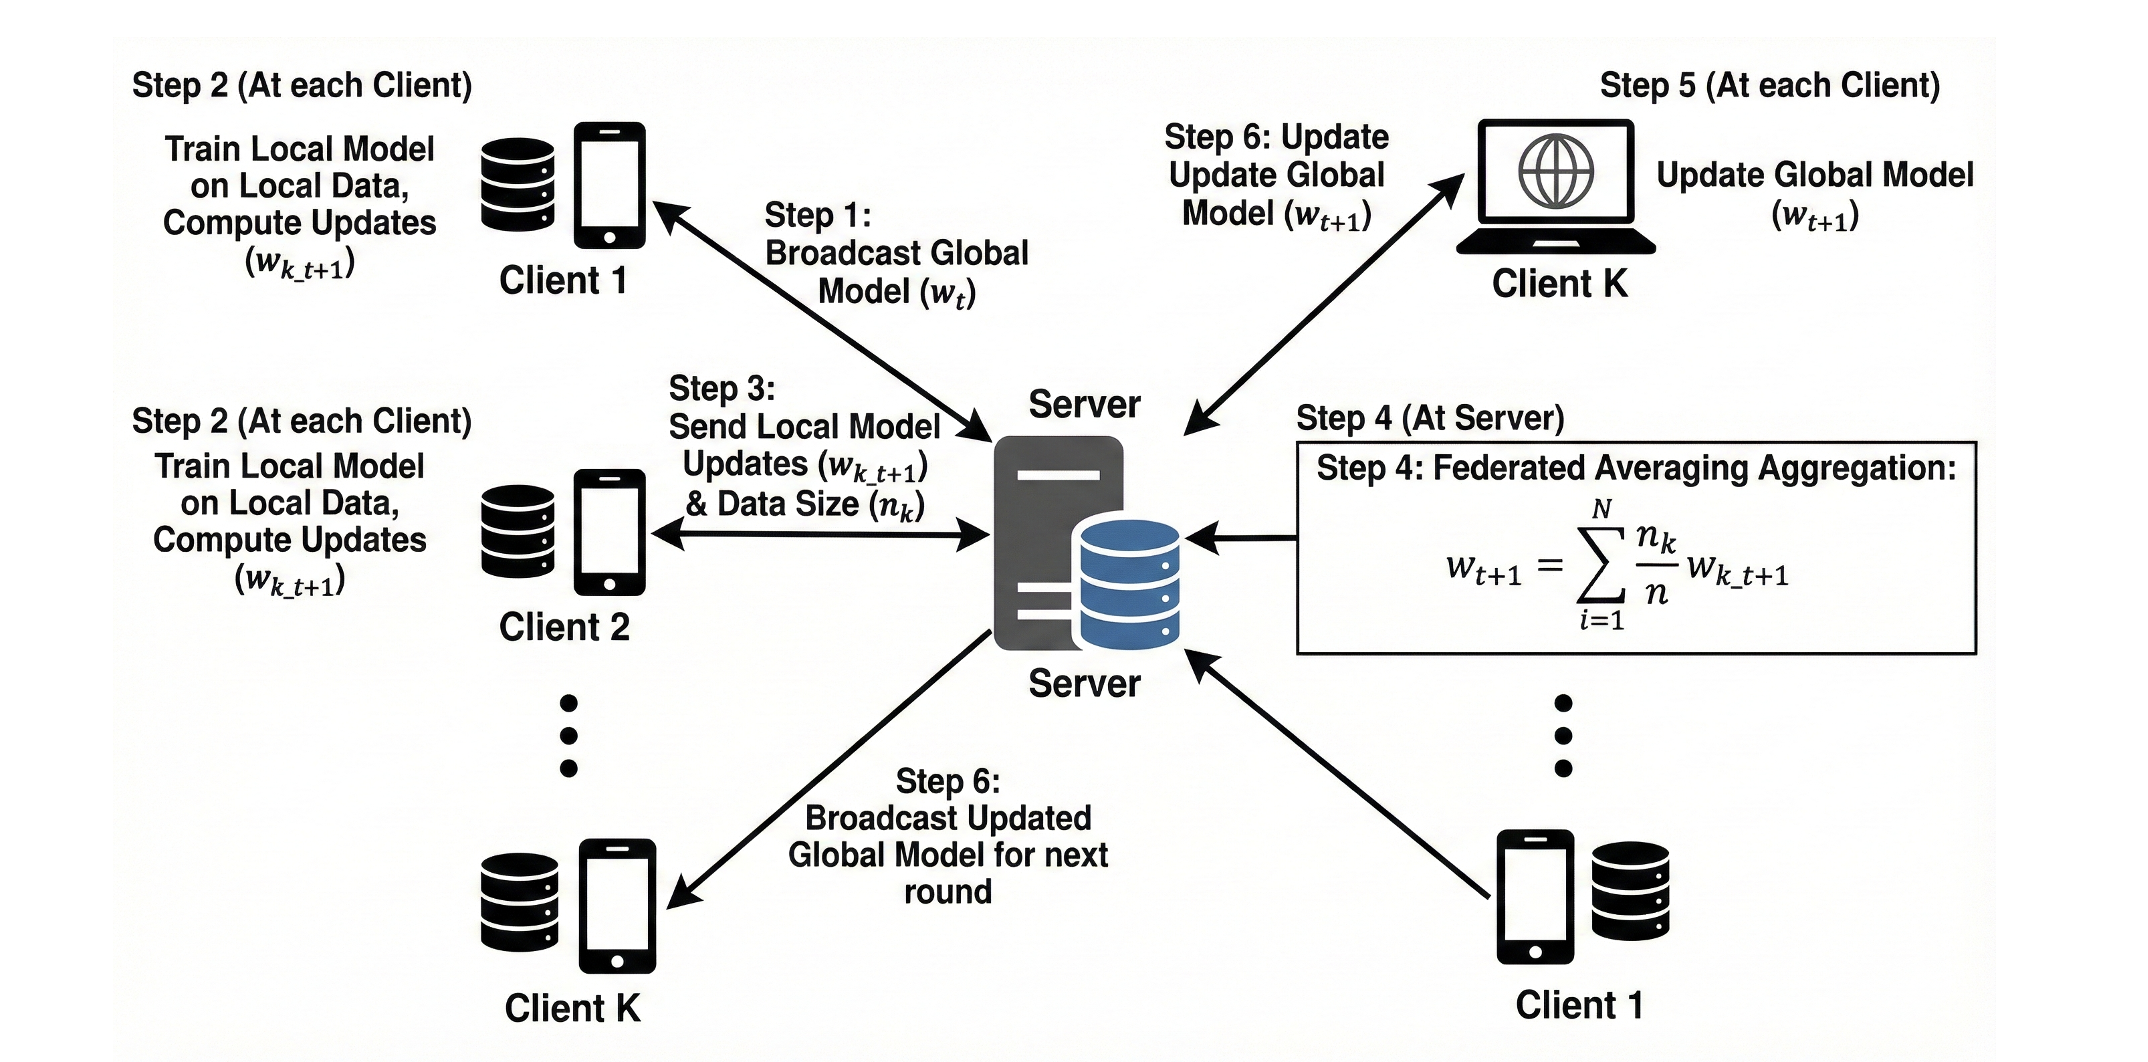
\includegraphics[width=0.7\textwidth]{img/fedavg_workflow.png}
        \captionof{figure}{Sơ đồ quy trình 4 bước của FedAvg: (1) Server phân phối, (2) Client cập nhật cục bộ, (3) Upload tham số, (4) Server tổng hợp \cite{McMahan2017}.}
        \label{fig:fedavg_workflow}
    \end{minipage}
\end{center}

\subsection{Phân tích Ưu và Nhược điểm}
\begin{itemize}
    \item \textbf{Ưu điểm:}
    \begin{itemize}
        \item \textbf{Hiệu quả truyền thông:} FedAvg giảm đáng kể tần suất giao tiếp so với SGD phân tán truyền thống. Thực nghiệm cho thấy FedAvg có thể giảm từ 10-100 lần số vòng lặp cần thiết để đạt độ chính xác tương đương trên các mô hình CNN \cite{McMahan2017}.
        \item \textbf{Tính riêng tư:} Dữ liệu thô được giữ lại hoàn toàn tại biên (edge devices).
        \item \textbf{Khả năng mở rộng:} Cơ chế chọn mẫu ngẫu nhiên (client sampling) cho phép hệ thống hoạt động tốt ngay cả khi số lượng thiết bị lên tới hàng triệu.
    \end{itemize}
    
    \item \textbf{Nhược điểm:}
    \begin{itemize}
        \item \textbf{Vấn đề Client Drift (Trôi dạt mô hình):} Đây là hạn chế lớn nhất. Trong môi trường dữ liệu Non-IID (phân phối dữ liệu khác nhau giữa các client), hàm tối ưu cục bộ $F_k(w)$ sẽ khác xa hàm tối ưu toàn cầu $f(w)$. Khi thực hiện nhiều bước cập nhật cục bộ ($E$ lớn), $w^k$ sẽ hội tụ về cực tiểu riêng của client đó thay vì cực tiểu chung, dẫn đến mô hình toàn cầu bị phân kỳ hoặc giảm độ chính xác \cite{McMahan2017}.
        \item \textbf{Tắc nghẽn do thiết bị chậm (Stragglers):} Quá trình tổng hợp phải chờ đợi client chậm nhất trong tập $S_t$ hoàn thành, gây lãng phí tài nguyên của các thiết bị nhanh hơn.
    \end{itemize}
\end{itemize}

\section{Thuật toán FedLWS (Federated Layer-wise Weight Shrinking)}
\label{sec:FedLWS}

\subsection{Tổng quan và Động lực nghiên cứu}
\textbf{Federated Learning with Layer-wise Weight Shrinking (FedLWS)}, được đề xuất bởi Shi và các cộng sự tại hội nghị ICLR 2025, là một phương pháp tối ưu hóa tiên tiến nhằm giải quyết vấn đề \textit{Client Drift} trong môi trường dữ liệu Non-IID \cite{Shi2025LWS}.

Động lực của FedLWS xuất phát từ một quan sát thực nghiệm sâu sắc về kiến trúc mạng nơ-ron sâu (Deep Neural Networks): "Độ nhạy cảm của các lớp mạng đối với sự không đồng nhất dữ liệu là không giống nhau".
\begin{itemize}
    \item Các lớp nông (Shallow layers - gần đầu vào): Thường học các đặc trưng cấp thấp (cạnh, góc, vân bề mặt) mang tính phổ quát, ít bị thay đổi giữa các client.
    \item Các lớp sâu (Deep layers - gần đầu ra): Chịu trách nhiệm phân loại dựa trên ngữ nghĩa cao cấp, do đó rất nhạy cảm và dễ bị lệch hướng (drift) khi dữ liệu cục bộ mất cân bằng nhãn (label distribution skew).
\end{itemize}

FedAvg thất bại trong việc nắm bắt sự tinh tế này vì nó áp dụng cơ chế trung bình cào bằng cho tất cả các lớp. FedLWS khắc phục điều này bằng cách áp dụng cơ chế "co trọng số" (weight shrinking) với tỷ lệ khác nhau cho từng lớp dựa trên độ ổn định của chúng.

\subsection{Cơ sở Toán học và Quy trình thực hiện}
Giả sử mô hình toàn cầu $w$ được cấu thành từ $L$ lớp mạng, ký hiệu là $\{w^1, w^2, ..., w^L\}$. Tại vòng giao tiếp $t$, sau khi các client thực hiện huấn luyện cục bộ và gửi cập nhật $\Delta w_k^t = w_k^{t+1} - w^t$ về máy chủ, FedLWS thực hiện quy trình tổng hợp 3 bước như sau:

{Bước 1: Tính toán Phương sai theo lớp (Layer-wise Variance)}
Máy chủ đo lường mức độ "bất đồng" giữa các client tại từng lớp mạng $l$ bằng cách tính phương sai của các vector cập nhật. Nếu các client cập nhật lớp $l$ theo các hướng quá khác nhau, phương sai sẽ cao, báo hiệu sự mất ổn định do dữ liệu Non-IID.
Công thức tính phương sai lớp $l$:
\begin{equation}
    \sigma_l^t = \frac{1}{K} \sum_{k=1}^{K} \left\| \Delta w_k^{l, t} - \overline{\Delta w^{l, t}} \right\|_2^2
\end{equation}
Trong đó $\overline{\Delta w^{l, t}}$ là trung bình cập nhật của lớp $l$.

{Bước 2: Xác định Hệ số Co (Shrinking Factor)}
Dựa trên phương sai $\sigma_l^t$, thuật toán tính toán một hệ số co $\alpha_l^t \in (0, 1]$ cho từng lớp. Nguyên tắc là: "Lớp nào biến động mạnh (phương sai lớn) thì co nhiều, lớp nào ổn định thì giữ nguyên".
Hàm tính hệ số co được đề xuất như sau:
\begin{equation}
    \alpha_l^t = \frac{1}{1 + \beta \cdot \exp(\gamma \cdot \sigma_l^t)}
\end{equation}
Trong đó $\beta$ và $\gamma$ là các siêu tham số kiểm soát độ nhạy của hàm co. Khi $\sigma_l^t \to 0$ (ổn định), $\alpha_l^t \to 1$ (giữ nguyên). Khi $\sigma_l^t$ lớn (bất ổn), $\alpha_l^t \to 0$ (giảm bớt sự đóng góp).

{Bước 3: Tổng hợp Thích ứng (Adaptive Aggregation)}
Máy chủ cập nhật mô hình toàn cầu bằng cách áp dụng hệ số co vào công thức trung bình trọng số. Thay vì cộng trực tiếp, các cập nhật sẽ được "làm mềm" (dampened) để tránh việc mô hình toàn cầu bị kéo lệch quá xa bởi các client cực đoan:
\begin{equation}
    w^{l, t+1} = w^{l, t} + \alpha_l^t \cdot \sum_{k=1}^{K} \frac{n_k}{n} \Delta w_k^{l, t}
\end{equation}

\begin{center}
    \begin{minipage}{\linewidth}
        \centering
        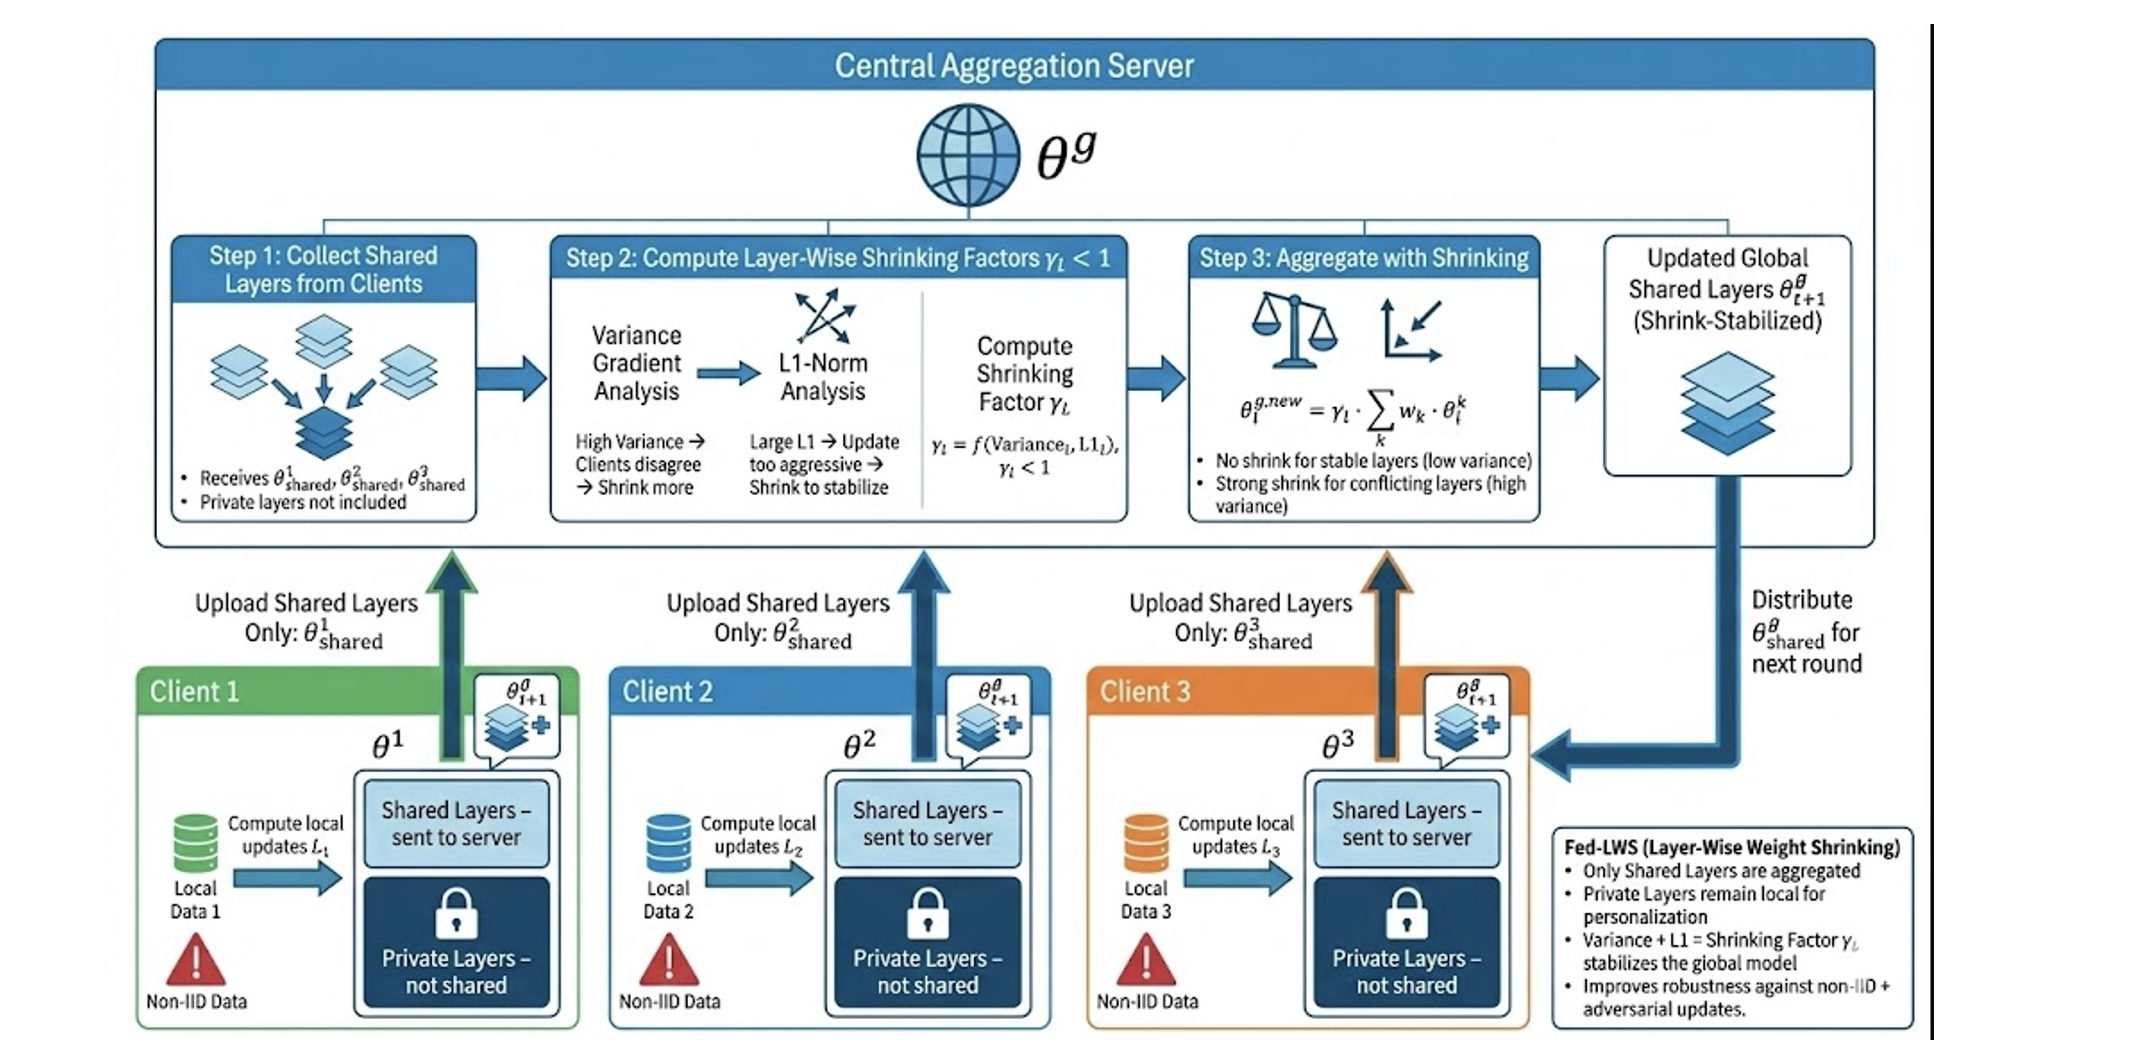
\includegraphics[width=0.85\textwidth]{img/fedlws_mechanism.png}
        \captionof{figure}{Cơ chế hoạt động của FedLWS: Các lớp sâu (gần output) có phương sai cập nhật lớn (màu đỏ) sẽ bị áp dụng hệ số co mạnh hơn để ổn định mô hình toàn cầu \cite{Shi2025LWS}.}
        \label{fig:fedlws_mechanism}
    \end{minipage}
\end{center}

\subsection{Phân tích Ưu và Nhược điểm}
\begin{itemize}
    \item \textbf{Ưu điểm:}
    \begin{itemize}
        \item \textbf{Cải thiện độ chính xác trên Non-IID:} Bằng cách kìm hãm các lớp nhạy cảm (thường là nguyên nhân chính gây Client Drift), FedLWS giúp mô hình hội tụ ổn định hơn và đạt độ chính xác cao hơn so với FedAvg (thực nghiệm cho thấy tăng ~2-3% trên CIFAR-10) \cite{Shi2025LWS}.
        \item \textbf{Không cần dữ liệu Proxy:} Khác với một số phương pháp yêu cầu server phải có một tập dữ liệu nhỏ để tinh chỉnh (như FedDF), FedLWS hoàn toàn dựa trên thống kê của trọng số mô hình, đảm bảo tính thực tế khi triển khai.
        \item \textbf{Chi phí truyền thông không đổi:} Không yêu cầu client gửi thêm bất kỳ thông tin phụ trợ nào ngoài tham số mô hình.
    \end{itemize}
    
    \item \textbf{Nhược điểm:}
    \begin{itemize}
        \item \textbf{Chi phí tính toán tại Server:} Máy chủ phải thực hiện tính toán phương sai và hệ số co cho từng lớp tại mỗi vòng lặp. Tuy nhiên, chi phí này là không đáng kể so với chi phí huấn luyện.
        \item \textbf{Thêm siêu tham số:} Việc lựa chọn $\beta, \gamma$ phù hợp có thể yêu cầu quá trình tinh chỉnh (tuning) dựa trên từng bộ dữ liệu cụ thể.
    \end{itemize}
\end{itemize}



\section{Thuật toán FedAWA (Federated Learning with Adaptive Weight Aggregation)}
\label{sec:FedAWA}

\subsection{Tổng quan và Động lực nghiên cứu}
\textbf{FedAWA (Federated Learning with Adaptive Weight Aggregation)}, được đề xuất bởi Shi và các cộng sự (2025), là một phương pháp tiếp cận mới nhằm giải quyết triệt để hạn chế của cơ chế trung bình trọng số dựa trên kích thước dữ liệu (sample-size based averaging) của FedAvg \cite{Shi2025AWA}.

Trong FedAvg, trọng số của một client ($n_k/n$) là cố định dựa trên số lượng mẫu dữ liệu mà nó sở hữu. Tuy nhiên, trong bối cảnh Non-IID, số lượng không đại diện cho chất lượng. Một client có lượng dữ liệu lớn nhưng bị lệch nhãn nghiêm trọng (ví dụ: chỉ chứa ảnh của 1 lớp duy nhất) có thể đóng góp một vector cập nhật "có hại", kéo mô hình toàn cầu lệch khỏi điểm tối ưu.

Động lực của FedAWA là xây dựng một cơ chế "Trọng số thích ứng theo chất lượng". Thuật toán tự động nhận diện và gán trọng số cao cho các client có hướng cập nhật tốt (đại diện cho phân phối chung), đồng thời giảm trọng số của các client bị lệch (bias), bất kể lượng dữ liệu của chúng là bao nhiêu.

\subsection{Cơ sở Toán học: Client Vector và Bài toán Tối ưu}
Để đánh giá chất lượng cập nhật mà không cần truy cập dữ liệu, FedAWA giới thiệu khái niệm \textbf{"Client Vector"}.

{Định nghĩa Client Vector}
Tại vòng giao tiếp $t$, sau khi client $k$ hoàn thành huấn luyện cục bộ và thu được tham số $\theta_k^{t+1}$, \textit{Client Vector} $\tau_k^t$ được định nghĩa là sự thay đổi của mô hình cục bộ so với mô hình toàn cầu ban đầu:
\begin{equation}
    \tau_k^t = \theta_k^{t+1} - \theta_g^t
\end{equation}
Về bản chất, $\tau_k^t$ đại diện cho hướng (direction) và độ lớn (magnitude) của gradient tích lũy mà client $k$ muốn áp dụng lên mô hình toàn cầu. Trong không gian tham số, các client có phân phối dữ liệu giống nhau sẽ sinh ra các Client Vector có hướng tương tự nhau \cite{Shi2025AWA}.

{Cơ chế Tối ưu hóa Trọng số (Adaptive Weight Optimization)}
Mục tiêu của FedAWA là tìm ra một bộ trọng số $\Lambda = \{\lambda_1, \lambda_2, ..., \lambda_K\}$ (với $\sum \lambda_k = 1, \lambda_k \ge 0$) sao cho vector tổng hợp toàn cầu $\tau_g = \sum \lambda_k \tau_k$ là "tốt nhất".

"Tốt nhất" ở đây được định nghĩa là vector tổng hợp phải giảm thiểu khoảng cách đến các vector thành phần (thể hiện sự đồng thuận) và duy trì tính ổn định. Máy chủ giải bài toán tối ưu hóa sau tại mỗi vòng lặp:
\begin{equation}
    \min_{\Lambda} \left( \sum_{k=1}^{K} \lambda_k \left\| \tau_k^t - \sum_{j=1}^{K} \lambda_j \tau_j^t \right\|_2^2 + \gamma \left\| \sum_{k=1}^{K} \lambda_k \tau_k^t \right\|_2^2 \right)
\end{equation}
Trong đó:
\begin{itemize}
    \item Số hạng thứ nhất: Đo lường phương sai của các client vector so với vector trung bình. Việc tối thiểu hóa số hạng này giúp loại bỏ các client ngoại lai (outliers) có hướng cập nhật quá khác biệt.
    \item Số hạng thứ hai: Là thành phần điều chuẩn (regularization) với hệ số $\gamma$, giúp kiểm soát độ lớn của bước cập nhật toàn cầu, tránh việc mô hình bị thay đổi quá đột ngột.
\end{itemize}

Sau khi giải bài toán tối ưu này (thường bằng phương pháp Frank-Wolfe hoặc Gradient Descent trên simplex), máy chủ thu được bộ trọng số tối ưu $\Lambda^*$ để cập nhật mô hình:
\begin{equation}
    \theta_g^{t+1} = \theta_g^t + \eta_g \sum_{k=1}^{K} \lambda_k^* \tau_k^t
\end{equation}

\begin{center}
    \begin{minipage}{\linewidth}
        \centering
        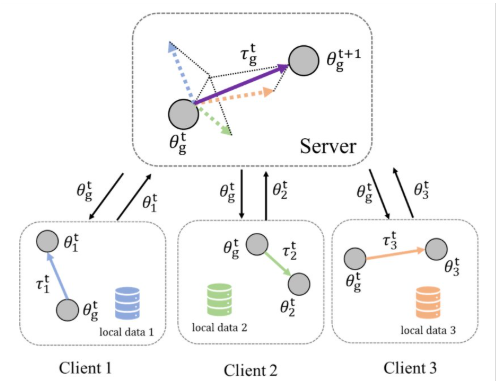
\includegraphics[width=0.8\textwidth]{img/fedawa_mechanism.png}
        \captionof{figure}{Minh họa cơ chế của FedAWA: Các Client Vector (mũi tên nhỏ) có hướng khác nhau do Non-IID. FedAWA tính toán vector tổng hợp tối ưu (mũi tên đậm) sao cho giảm thiểu sự phân kỳ, thay vì chỉ cộng trung bình \cite{Shi2025AWA}.}
        \label{fig:FedAWA}
    \end{minipage}
\end{center}

\subsection{Phân tích Ưu và Nhược điểm}
\begin{itemize}
    \item \textbf{Ưu điểm:}
    \begin{itemize}
        \item \textbf{Khắc phục triệt để Client Drift:} Bằng cách gán trọng số thấp cho các client có vector cập nhật lệch hướng (thường là các client có dữ liệu cực đoan), FedAWA giúp mô hình hội tụ ổn định hơn nhiều so với FedAvg.
        \item \textbf{Công bằng hơn:} Trọng số được quyết định bởi chất lượng đóng góp thay vì số lượng dữ liệu. Điều này đặc biệt hữu ích khi một số client có rất nhiều dữ liệu nhưng chất lượng thấp (rác, nhiễu).
        \item \textbf{Không cần tham số phụ:} Thuật toán hoạt động hoàn toàn dựa trên trọng số mô hình gửi về, không yêu cầu client gửi thêm thống kê loss hay gradient.
    \end{itemize}
    
    \item \textbf{Nhược điểm:}
    \begin{itemize}
        \item \textbf{Chi phí tính toán tại Server cao:} Việc giải bài toán tối ưu hóa tìm $\Lambda^*$ tại mỗi vòng lặp phức tạp hơn nhiều so với phép tính trung bình đơn giản ($O(1)$) của FedAvg. Khi số lượng client $K$ rất lớn, bước này có thể tạo ra nút thắt cổ chai về thời gian xử lý.
    \end{itemize}
\end{itemize}



\section{Thuật toán FedNolowe (Federated Normalized Loss-based Weighted Aggregation)}
\label{sec:FedNolowe}

\subsection{Tổng quan và Động lực nghiên cứu}
\textbf{FedNolowe}, được đề xuất bởi Lê và các cộng sự (2025), đại diện cho một hướng tiếp cận dựa trên hiệu suất (performance-based aggregation) thay vì dựa trên khối lượng dữ liệu \cite{Le2025}.

Động lực của thuật toán xuất phát từ một thực tế trong Học máy liên kết: "Số lượng dữ liệu không đồng nghĩa với chất lượng mô hình". Trong thuật toán FedAvg truyền thống, một client sở hữu lượng dữ liệu lớn nhưng chứa nhiều nhiễu (noisy data) hoặc nhãn sai (incorrect labels) vẫn được gán trọng số cao ($n_k/n$). Điều này khiến mô hình toàn cầu bị "đầu độc" bởi các tri thức sai lệch, dẫn đến quá trình hội tụ không ổn định.

FedNolowe giải quyết vấn đề này bằng giả định: \textit{Giá trị hàm mất mát (Loss value) trên tập dữ liệu cục bộ là thước đo đáng tin cậy nhất cho mức độ "phù hợp" của dữ liệu client đối với tác vụ hiện tại}. Một client có loss thấp nghĩa là mô hình cục bộ đã học tốt, và ngược lại. Do đó, FedNolowe đề xuất cơ chế gán trọng số tỷ lệ nghịch với giá trị loss đã được chuẩn hóa.

\subsection{Cơ chế Chuẩn hóa Loss hai giai đoạn (Two-stage Loss Normalization)}
Quy trình cốt lõi của FedNolowe nằm ở việc chuyển đổi giá trị Loss thô (Raw Loss) từ các client thành trọng số tổng hợp $\alpha_k$. Quá trình này được thực hiện qua 2 giai đoạn toán học chặt chẽ:

{Giai đoạn 1: Chuẩn hóa Quy mô (Scale Normalization)}
Giả sử tại vòng $t$, có tập client tham gia $S_t$. Mỗi client $k$ gửi về máy chủ giá trị loss trung bình cục bộ $\mathcal{L}_k^t$.
Do giá trị loss có thể dao động trong khoảng rất rộng tùy thuộc vào batch size và dữ liệu, máy chủ trước tiên thực hiện chuẩn hóa L1 để đưa loss của tất cả client về cùng một thang đo tỷ lệ (từ 0 đến 1):
\begin{equation}
    \tilde{\mathcal{L}}_k^t = \frac{\mathcal{L}_k^t}{\sum_{j \in S_t} \mathcal{L}_j^t}
\end{equation}
Tại đây, $\tilde{\mathcal{L}}_k^t$ đại diện cho "tỷ trọng sai số" mà client $k$ đóng góp vào tổng sai số của hệ thống.

{Giai đoạn 2: Nghịch đảo và Tái chuẩn hóa (Inversion \& Re-normalization)}
Mục tiêu của chúng ta là: \textbf{Loss càng cao $\to$ Trọng số càng thấp}. Do đó, thuật toán sử dụng phép nghịch đảo dựa trên hiệu số (subtraction-based inversion) để tránh các vấn đề về số học (như chia cho 0).
Giá trị điểm số (score) của client $k$ được tính là phần bù của loss chuẩn hóa: $1 - \tilde{\mathcal{L}}_k^t$.

Cuối cùng, trọng số tổng hợp $\alpha_k^t$ được xác định bằng cách tái chuẩn hóa các điểm số này sao cho tổng trọng số bằng 1:
\begin{equation}
    \alpha_k^t = \frac{1 - \tilde{\mathcal{L}}_k^t}{\sum_{j \in S_t} (1 - \tilde{\mathcal{L}}_j^t)}
\end{equation}
Công thức này đảm bảo rằng các client có loss thấp (hiệu suất tốt) sẽ có $\alpha_k^t$ lớn, đóng góp nhiều hơn vào mô hình toàn cầu. Ngược lại, các client có loss cao bất thường (có thể do dữ liệu nhiễu hoặc tấn công) sẽ bị gán trọng số rất nhỏ, giảm thiểu tác động tiêu cực.

\subsection{Quy trình thực hiện tổng thể}
Tại mỗi vòng giao tiếp $t$:
\begin{enumerate}
    \item \textbf{Huấn luyện và Báo cáo:} Client $k$ thực hiện huấn luyện cục bộ để cập nhật trọng số $w_k^{t+1}$, đồng thời tính toán loss trung bình $\mathcal{L}_k^t$ trên tập dữ liệu của mình. Client gửi cả $w_k^{t+1}$ và $\mathcal{L}_k^t$ về server.
    
    \item \textbf{Tính toán Trọng số:} Server thu thập các giá trị loss, thực hiện quy trình chuẩn hóa 2 giai đoạn như trên để tìm ra bộ trọng số $\{\alpha_k^t\}$.
    
    \item \textbf{Tổng hợp Mô hình:} Server cập nhật mô hình toàn cầu mới:
    \begin{equation}
        w^{t+1} = \sum_{k \in S_t} \alpha_k^t w_k^{t+1}
    \end{equation}
\end{enumerate}
\begin{center}
    \begin{minipage}{\linewidth}
        \centering
        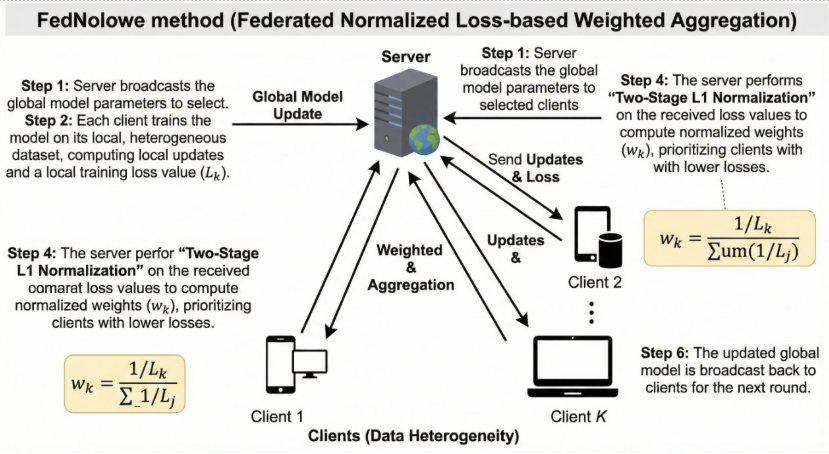
\includegraphics[width=0.85\textwidth]{img/fednolowe_process.png}
        \captionof{figure}{Sơ đồ minh họa quy trình của FedNolowe: Từ Loss cục bộ $\mathcal{L}_k$ được chuyển đổi qua 2 bước chuẩn hóa để tạo ra trọng số $\alpha_k$ tối ưu \cite{Le2025}.}
        \label{fig:fednolowe_process}
    \end{minipage}
\end{center}

\subsection{Phân tích Ưu và Nhược điểm}
\begin{itemize}
    \item \textbf{Ưu điểm:}
    \begin{itemize}
        \item \textbf{Kháng nhiễu tốt (Robustness):} FedNolowe tự động loại bỏ tác động của các client "kém chất lượng" (loss cao), giúp mô hình ổn định hơn trước dữ liệu nhiễu hoặc phân phối Non-IID cực đoan.
        \item \textbf{Hiệu quả tính toán:} Quy trình tính toán trọng số $\alpha_k$ cực kỳ đơn giản (độ phức tạp $O(K)$), nhanh hơn nhiều so với việc giải bài toán tối ưu của FedAWA.
        \item \textbf{Dễ tích hợp:} Có thể áp dụng ngay lập tức vào bất kỳ kiến trúc FL nào mà không cần thay đổi cấu trúc mô hình.
    \end{itemize}
    
    \item \textbf{Nhược điểm:}
    \begin{itemize}
        \item \textbf{Nguy cơ về quyền riêng tư:} Việc gửi giá trị Loss về server có thể rò rỉ một phần thông tin về độ khó của dữ liệu cục bộ (mặc dù ít nghiêm trọng hơn gửi gradient).
        \item \textbf{Phụ thuộc vào tính trung thực:} Nếu một client gian dối báo cáo loss giả mạo (rất thấp) mặc dù không học gì, nó có thể chiếm quyền kiểm soát mô hình toàn cầu (Loss poisoning attack).
    \end{itemize}
\end{itemize}

\section{Thuật toán FedProto (Federated Prototype Learning)}
\label{sec:FedProto}

\subsection{Tổng quan và Động lực nghiên cứu}
\textbf{FedProto (Federated Prototype Learning)}, được giới thiệu bởi Tan và các cộng sự tại hội nghị AAAI 2022, đại diện cho một bước chuyển mình quan trọng trong tư duy thiết kế hệ thống Học máy liên kết \cite{Tan2022}.

Các thuật toán truyền thống như FedAvg, FedLWS hay FedAWA đều dựa trên một giả định cứng nhắc: "Tất cả các client phải sử dụng cùng một kiến trúc mạng nơ-ron (Model Isomorphism)". Tuy nhiên, trong thực tế, các thiết bị tham gia mạng lưới (IoT, điện thoại, máy chủ) có năng lực phần cứng rất khác nhau. Ép buộc một thiết bị IoT yếu ớt chạy cùng mô hình ResNet-50 với một máy chủ mạnh mẽ là điều không khả thi.

FedProto ra đời để giải quyết vấn đề "Tính không đồng nhất về mô hình" (Model Heterogeneity). Thay vì trao đổi tham số mô hình (gradients/weights) - vốn yêu cầu kiến trúc phải giống hệt nhau để thực hiện phép cộng, FedProto đề xuất trao đổi "Tri thức lớp" (Class Prototypes). Điều này cho phép các client sử dụng các mô hình khác nhau (ResNet, CNN, MobileNet...) nhưng vẫn có thể cộng tác học tập thông qua ngôn ngữ chung là các vector đặc trưng lớp.

\subsection{Cơ sở Toán học: Prototype và Cơ chế giao tiếp}

{Định nghĩa Prototype (Mẫu hình)}
Trong FedProto, một \textit{Prototype} của lớp $j$, ký hiệu là $C^{(j)}$, được định nghĩa là vector trung bình của các biểu diễn đặc trưng (embedding vectors) của tất cả dữ liệu thuộc lớp đó.
Giả sử client $k$ có bộ trích xuất đặc trưng (Feature Extractor) $f_k(\cdot)$. Với tập dữ liệu cục bộ $D_{k,j}$ thuộc lớp $j$, prototype cục bộ được tính như sau:
\begin{equation}
    C_k^{(j)} = \frac{1}{|D_{k,j}|} \sum_{(x,y) \in D_{k,j}} f_k(x)
\end{equation}
Prototype này đóng vai trò là "đại diện ngữ nghĩa" cho lớp $j$ tại client $k$.

{Cơ chế Học dựa trên Prototype (Prototype-based Learning)}
Quy trình tối ưu hóa của FedProto không cập nhật trọng số trực tiếp từ server. Thay vào đó, nó sử dụng các Global Prototypes để hướng dẫn quá trình huấn luyện cục bộ thông qua một hàm mất mát điều chuẩn (Regularization Loss).

Hàm mục tiêu cục bộ tại client $k$ được thiết lập như sau:
\begin{equation}
    \min_{\theta_k} \mathcal{L}_{total} = \mathcal{L}_{CE}(\hat{y}, y) + \lambda \cdot \mathcal{L}_{proto}
\end{equation}
Trong đó:
\begin{itemize}
    \item $\mathcal{L}_{CE}$: Hàm mất mát Cross-Entropy tiêu chuẩn để phân loại đúng.
    \item $\mathcal{L}_{proto}$: Hàm mất mát khoảng cách (thường là L2 distance), ép buộc đặc trưng của dữ liệu cục bộ $f_k(x_i)$ phải tiến gần về phía Prototype toàn cầu $\bar{C}^{(y_i)}$ tương ứng với nhãn $y_i$:
    \begin{equation}
        \mathcal{L}_{proto} = \frac{1}{|D_k|} \sum_{(x_i, y_i) \in D_k} \| f_k(x_i) - \bar{C}^{(y_i)} \|_2^2
    \end{equation}
\end{itemize}

\subsection{Quy trình thực hiện thuật toán}
Quy trình của FedProto khác biệt hoàn toàn so với dòng họ FedAvg do không có bước "cộng trọng số".

\begin{enumerate}
    \item \textbf{Huấn luyện và Tính toán Prototype:} Client $k$ huấn luyện mô hình riêng của mình, sau đó tính toán bộ prototype cục bộ $C_k = \{C_k^{(1)}, ..., C_k^{(M)}\}$ cho các lớp dữ liệu mà nó sở hữu.
    
    \item \textbf{Tải lên (Upload):} Client gửi bộ vector $C_k$ về máy chủ.
    \textit{Lưu ý:} Kích thước của vector prototype nhỏ hơn hàng ngàn lần so với bộ tham số mô hình, giúp tiết kiệm băng thông cực lớn.
    
    \item \textbf{Tổng hợp (Aggregation):} Server tổng hợp các prototype cục bộ cùng lớp để tạo ra Prototype toàn cầu:
    \begin{equation}
        \bar{C}^{(j)} = \frac{1}{|S_j|} \sum_{k \in S_j} C_k^{(j)}
    \end{equation}
    với $S_j$ là tập các client có sở hữu dữ liệu lớp $j$.
    
    \item \textbf{Phân phối (Broadcast):} Server gửi bộ Prototype toàn cầu $\bar{C} = \{\bar{C}^{(1)}, ...\}$ về cho các client để sử dụng cho vòng huấn luyện tiếp theo (tính toán $\mathcal{L}_{proto}$).
\end{enumerate}

\begin{center}
    \begin{minipage}{\linewidth}
        \centering
        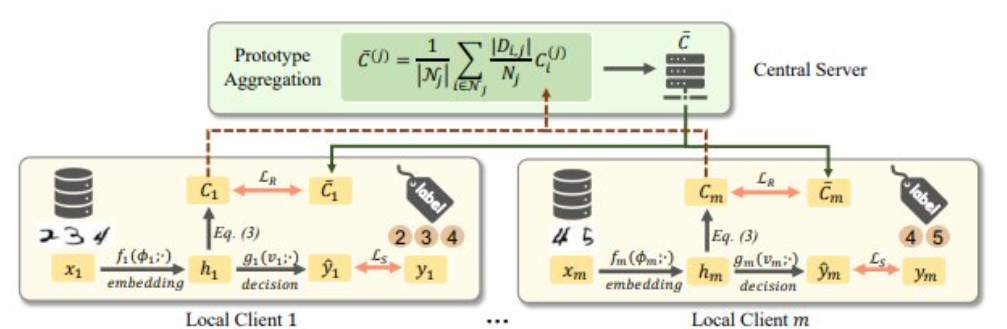
\includegraphics[width=0.9\textwidth]{img/fedproto_framework.png}
        \captionof{figure}{Kiến trúc FedProto: Các client với mô hình khác nhau (Heterogeneous Models) giao tiếp bằng cách gửi các vector Prototype màu sắc về Server thay vì gửi tham số mô hình \cite{Tan2022}.}
        \label{fig:FedProto}
    \end{minipage}
\end{center}
\subsection{Phân tích Ưu và Nhược điểm}
\begin{itemize}
    \item \textbf{Ưu điểm:}
    \begin{itemize}
        \item \textbf{Hỗ trợ Mô hình không đồng nhất:} Đây là ưu điểm độc nhất. Client mạnh có thể dùng ResNet-50, client yếu dùng MobileNetV3, chúng vẫn học được từ nhau.
        \item \textbf{Siêu tiết kiệm băng thông:} Vector prototype (ví dụ: 10 lớp $\times$ 512 chiều) nhỏ hơn rất nhiều so với mô hình (triệu tham số).
        \item \textbf{Bảo mật cao:} Không gửi tham số mô hình đồng nghĩa với việc cực khó để khôi phục lại cấu trúc mạng hay dữ liệu gốc (Gradient Inversion Attack trở nên vô hiệu).
    \end{itemize}
    
    \item \textbf{Nhược điểm:}
    \begin{itemize}
        \item \textbf{Phụ thuộc vào Không gian đặc trưng:} Thuật toán chỉ hoạt động tốt khi các mô hình khác nhau trích xuất ra không gian đặc trưng (embedding space) có cùng số chiều.
        \item \textbf{Hiệu suất trên IID:} Trong trường hợp lý tưởng (IID, mô hình giống nhau), FedProto thường có độ chính xác thấp hơn FedAvg do không tận dụng được việc chia sẻ tham số chi tiết.
        \item \textbf{Vấn đề Missing Class:} Nếu một lớp dữ liệu không xuất hiện ở bất kỳ client nào trong vòng đó, Prototype toàn cầu của lớp đó sẽ không được cập nhật.
    \end{itemize}
\end{itemize}

\chapter{Phương pháp đề xuất: FedSecL}
\label{ch:fedcil}
Trong chương này, nhóm đề xuất phương pháp \textbf{FedSecL (Federated Secure Loss-based Aggregation)}. Đây là một phiên bản cải tiến dựa trên nền tảng của thuật toán FedNolowe, bổ sung cơ chế \textbf{"Lớp lọc bảo mật"} (Security Filtering Layer) nhằm khắc phục nhược điểm về an toàn thông tin, đảm bảo sự ổn định của mô hình trước các hành vi gian lận hoặc tấn công từ client.

\section{Động lực và Cơ sở ý tưởng}
\label{sec:motivation}

\subsection{Hạn chế của phương pháp dựa trên Loss (FedNolowe)}
Như đã phân tích ở Chương 2, các phương pháp tổng hợp trọng số dựa trên hàm mất mát (như FedNolowe) rất hiệu quả trong việc xử lý dữ liệu Non-IID. Nguyên lý của chúng là: \textit{"Client nào có Loss thấp (học tốt) thì được gán trọng số cao"}.

Tuy nhiên, cơ chế này tồn tại một lỗ hổng bảo mật nghiêm trọng gọi là \textbf{Tấn công đầu độc mô hình (Model Poisoning) thông qua gian lận Loss}:
\begin{itemize}
    \item \textbf{Kịch bản tấn công:} Một client ác ý (Malicious Client) có thể không thực hiện huấn luyện (Free-rider) hoặc cố tình phá hoại, nhưng lại báo cáo về Server một giá trị Loss rất nhỏ (giả mạo).
    \item \textbf{Hậu quả:} Thuật toán sẽ lầm tưởng client này là "học sinh xuất sắc" và gán cho nó trọng số cực lớn. Kết quả là mô hình toàn cục bị điều hướng theo tham số sai lệch của kẻ tấn công, dẫn đến sụp đổ độ chính xác.
\end{itemize}

\subsection{Ý tưởng cải tiến: "Tin tưởng nhưng Xác minh"}
Để giải quyết vấn đề này mà vẫn giữ được ưu điểm xử lý Non-IID, nhóm đề xuất bổ sung một Lớp chặn (Blocking Layer) tại Server.

Ý tưởng cốt lõi là sử dụng các \textbf{Thống kê mô tả (Descriptive Statistics)} của tập hợp các giá trị Loss gửi về để xác định ngưỡng an toàn. Bất kỳ giá trị Loss nào nằm ngoài vùng phân phối bình thường (quá cao hoặc quá thấp một cách đáng ngờ) sẽ bị coi là bất thường (Anomaly) và bị loại bỏ khỏi quá trình tổng hợp.

\section{Thiết kế thuật toán FedSecL}
\label{sec:design}

Phương pháp FedSecL bao gồm hai thành phần chính: Cơ chế phát hiện bất thường và Cơ chế tổng hợp trọng số an toàn.

\subsection{Cơ chế "Lớp chặn" (Security Filtering Layer)}
Giả sử tại vòng $t$, Server nhận được tập hợp các giá trị loss từ $K$ client: $\mathcal{L}^t = \{\mathcal{L}_1^t, \mathcal{L}_2^t, ..., \mathcal{L}_K^t\}$.

Thay vì dùng trực tiếp các giá trị này, Server thực hiện quy trình lọc 3 bước:

\begin{enumerate}
    \item \textbf{Bước 1: Tính toán tham số thống kê.}
    nhóm sử dụng \textit{Trung vị (Median)} thay vì Trung bình (Mean) để làm mốc chuẩn, vì trung vị ít bị ảnh hưởng bởi các giá trị ngoại lai (outliers).
    \begin{equation}
        \mu_{med}^t = \text{Median}(\mathcal{L}^t)
    \end{equation}
    
    \item \textbf{Bước 2: Xác định ngưỡng chặn (Thresholding).}
    Một dải an toàn (Safe Zone) được thiết lập dựa trên độ lệch tuyệt đối trung vị (MAD - Median Absolute Deviation):
    \begin{equation}
        \text{MAD}^t = \text{Median}(|\mathcal{L}_i^t - \mu_{med}^t|)
    \end{equation}
    Ngưỡng chặn được xác định là: $[\mu_{med}^t - \gamma \cdot \text{MAD}^t, \mu_{med}^t + \gamma \cdot \text{MAD}^t]$, với $\gamma$ là hệ số kiểm soát độ chặt chẽ (thường chọn $\gamma=2$ hoặc $3$).

    \item \textbf{Bước 3: Sàng lọc Client.}
    Bất kỳ Client $k$ nào có giá trị $\mathcal{L}_k^t$ nằm ngoài khoảng an toàn trên sẽ bị đưa vào danh sách đen (Blacklist) trong vòng này và trọng số $\alpha_k$ bị gán bằng 0.
    \begin{itemize}
        \item $\mathcal{L}_k^t$ quá thấp $\rightarrow$ Nghi vấn gian lận giả mạo loss.
        \item $\mathcal{L}_k^t$ quá cao $\rightarrow$ Nghi vấn dữ liệu rác hoặc tấn công phá hoại.
    \end{itemize}
\end{enumerate}

\subsection{Cơ chế Tổng hợp Trọng số (Weighted Aggregation)}
Sau khi đi qua lớp chặn, tập hợp các client hợp lệ $S_{valid}$ sẽ được tính toán trọng số theo công thức chuẩn hóa nghịch đảo (tương tự FedNolowe nhưng an toàn hơn):

\begin{equation}
    \alpha_k^t = \frac{\exp(-\mathcal{L}_k^t)}{\sum_{j \in S_{valid}} \exp(-\mathcal{L}_j^t)}
\end{equation}
nhóm sử dụng hàm mũ $\exp(-x)$ để chuyển đổi Loss thành trọng số, giúp tăng độ mượt mà và tránh các lỗi chia cho 0.

\section{Quy trình thực hiện tổng thể}
\label{sec:workflow}

Quy trình hoạt động của FedSecL tại mỗi vòng giao tiếp diễn ra như sau:

\begin{center}
    \begin{minipage}{\linewidth}
        \centering
        \includegraphics[width=0.9\textwidth]{img/fedsecl_workflow.png}
        \captionof{figure}{Sơ đồ quy trình hoạt động của FedSecL với lớp màng lọc bảo mật tại Server.}
        \label{fig:fedsecl_workflow}
    \end{minipage}
\end{center}

\begin{itemize}
    \item \textbf{Bước 1 (Client):} Client tải mô hình toàn cầu, huấn luyện cục bộ trên dữ liệu riêng. Sau đó gửi về Server hai thông tin: Tham số mô hình $w_k$ và Giá trị Loss $\mathcal{L}_k$.
    
    \item \textbf{Bước 2 (Server - Lọc):} Server thu thập toàn bộ Loss, tính toán Trung vị và MAD. Các Loss bất thường bị phát hiện và loại bỏ.
    
    \item \textbf{Bước 3 (Server - Tính trọng số):} Với các client vượt qua lớp lọc, Server tính trọng số $\alpha_k$ dựa trên Loss của họ.
    
    \item \textbf{Bước 4 (Server - Tổng hợp):} Cập nhật mô hình toàn cầu mới:
    \begin{equation}
        w_{global} = \sum_{k \in S_{valid}} \alpha_k \cdot w_k
    \end{equation}
\end{itemize}

\section{Thảo luận về Ưu điểm}
Phương pháp FedSecL mang lại sự cân bằng giữa hiệu suất và an toàn:
\begin{enumerate}
    \item \textbf{Khả năng kháng nhiễu Non-IID:} Kế thừa ưu điểm của việc dùng Loss để đánh giá chất lượng dữ liệu, giúp mô hình hội tụ tốt hơn FedAvg.
    \item \textbf{Tính bảo mật cao:} Lớp chặn thống kê giúp loại bỏ hiệu quả các tấn công "Loss Spoofing" (giả mạo loss) và giảm thiểu tác động của các client chứa dữ liệu rác.
    \item \textbf{Độ phức tạp thấp:} Việc tính toán Trung vị và MAD rất đơn giản ($O(K \log K)$), không làm tăng đáng kể thời gian huấn luyện như các phương pháp mã hóa phức tạp hay Causal Learning.
\end{enumerate}

\chapter{Phương pháp thực hiện}
\label{c:phuongphapthuchien}
Chương này trình bày phương pháp nghiên cứu được áp dụng để phân tích và đánh giá các thuật toán tổng hợp trọng số tiên tiến trong Federated Learning. Nghiên cứu tập trung vào việc so sánh hiệu quả của 5 thuật toán chính: FedAvg, FedLWS, FedAWA, FedNolowe và FedProto thông qua phân tích lý thuyết và kết quả thực nghiệm từ các công bố khoa học.

\section{Phát biểu bài toán}

Trong môi trường Federated Learning, bài toán tổng hợp trọng số (Weight Aggregation) đóng vai trò then chốt trong việc kết hợp các cập nhật từ nhiều client để tạo ra mô hình toàn cầu tối ưu. Bài toán được phát biểu như sau:

\textbf{Đầu vào (Input):}
\begin{itemize}
    \item Hệ thống gồm $K$ clients, mỗi client $k$ có tập dữ liệu cục bộ $\mathcal{D}_k$ với kích thước $n_k$.
    \item Mô hình toàn cầu ban đầu với tham số $w_t$ tại vòng giao tiếp thứ $t$.
    \item Các cập nhật mô hình cục bộ $w_k^{t+1}$ sau khi client $k$ huấn luyện trên dữ liệu của mình.
    \item Dữ liệu phân tán có tính chất Non-IID (không đồng nhất về phân phối).
\end{itemize}

\textbf{Đầu ra (Output):}
\begin{itemize}
    \item Mô hình toàn cầu cập nhật $w_{t+1}$ được tổng hợp từ các mô hình cục bộ.
    \item Bộ trọng số tối ưu $\{\alpha_1, \alpha_2, ..., \alpha_K\}$ hoặc $\{\lambda_1, \lambda_2, ..., \lambda_K\}$ để kết hợp các cập nhật cục bộ.
\end{itemize}

\textbf{Mục tiêu:}
\begin{equation}
    w_{t+1} = \sum_{k=1}^{K} \alpha_k w_k^{t+1}
\end{equation}

Sao cho mô hình toàn cầu $w_{t+1}$ đạt được:
\begin{enumerate}
    \item Độ chính xác cao trên dữ liệu kiểm thử.
    \item Khả năng hội tụ nhanh và ổn định.
    \item Khả năng xử lý tốt dữ liệu Non-IID.
\end{enumerate}

\section{Phương pháp nghiên cứu}

Đề tài áp dụng phương pháp nghiên cứu kết hợp giữa nghiên cứu tài liệu và phân tích so sánh dựa trên kết quả thực nghiệm từ các công bố khoa học.

\subsection{Nghiên cứu tài liệu}

Quy trình nghiên cứu tài liệu được thực hiện theo các bước sau:

\begin{enumerate}
    \item \textbf{Thu thập tài liệu:}
    \begin{itemize}
        \item Tìm kiếm các bài báo khoa học từ các hội nghị và tạp chí uy tín: NeurIPS, ICML, ICLR, CVPR, AAAI.
        \item Tập trung vào các công trình được công bố từ năm 2022 đến 2025.
        \item Sử dụng các từ khóa: "Federated Learning", "Weight Aggregation", "Non-IID", "FedAvg", "FedLWS", "FedAWA", "FedNolowe", "FedProto".
    \end{itemize}
    
    \item \textbf{Phân loại và lựa chọn:}
    \begin{itemize}
        \item Phân loại các thuật toán theo cơ chế tổng hợp: dựa trên kích thước dữ liệu, loss, gradient, prototype.
        \item Lựa chọn 5 thuật toán đại diện: FedAvg (baseline), FedLWS, FedAWA, FedNolowe, FedProto.
    \end{itemize}
    
    \item \textbf{Phân tích chuyên sâu:}
    \begin{itemize}
        \item Phân tích cơ sở toán học của từng thuật toán.
        \item Xác định ưu điểm, nhược điểm và điều kiện áp dụng.
        \item So sánh độ phức tạp tính toán và yêu cầu băng thông.
    \end{itemize}
\end{enumerate}

\subsection{Phân tích so sánh}

Các thuật toán được so sánh dựa trên các tiêu chí sau:

\begin{table}[ht]
    \centering
    \caption{Các tiêu chí so sánh thuật toán}
    \label{tab:tieuchi}
    \renewcommand{\arraystretch}{1.3}
    \begin{tabular}{|l|p{10cm}|}
        \hline
        \textbf{Tiêu chí} & \textbf{Mô tả} \\
        \hline
        Độ chính xác & Accuracy trên tập kiểm thử (test accuracy) \\
        \hline
        Tốc độ hội tụ & Số vòng giao tiếp (communication rounds) cần thiết để đạt accuracy mục tiêu \\
        \hline
        Độ ổn định & Phương sai của accuracy qua các vòng huấn luyện \\
        \hline
        Khả năng xử lý Non-IID & Hiệu suất với dữ liệu Non-IID (Dirichlet $\alpha = 0.1$) và IID ($\alpha = 100$) \\
        \hline
        Độ phức tạp tính toán & Chi phí tính toán trên server và client \\
        \hline
        Yêu cầu băng thông & Kích thước dữ liệu cần truyền giữa client và server \\
        \hline
    \end{tabular}
\end{table}

\section{Thiết kế thực nghiệm}

Mặc dù đề tài này tập trung vào nghiên cứu lý thuyết và phân tích kết quả từ các công bố, nhóm mô tả thiết kế thực nghiệm chuẩn được sử dụng trong các nghiên cứu gốc để đánh giá các thuật toán.

\subsection{Bộ dữ liệu}

Các thuật toán được đánh giá trên hai bộ dữ liệu phổ biến:

\begin{itemize}
    \item \textbf{MNIST}~\cite{lecun1998mnist}: 
    \begin{itemize}
        \item 60,000 ảnh huấn luyện và 10,000 ảnh kiểm thử.
        \item 10 lớp chữ số viết tay (0-9).
        \item Kích thước ảnh: $28 \times 28$ pixels, grayscale.
    \end{itemize}
    

    \item \textbf{CIFAR-10}~\cite{krizhevsky2009cifar}:
    \begin{itemize}
        \item 50,000 ảnh huấn luyện và 10,000 ảnh kiểm thử.
        \item 10 lớp đối tượng (máy bay, ô tô, chim, mèo, v.v.).
        \item Kích thước ảnh: $32 \times 32$ pixels, RGB.
    \end{itemize}
\end{itemize}

\subsection{Thiết lập phân phối Non-IID}

Để mô phỏng tính không đồng nhất của dữ liệu trong thực tế, các nghiên cứu thường sử dụng phân phối Dirichlet để phân chia dữ liệu cho các client:

\begin{equation}
    p_k \sim \text{Dir}(\alpha)
\end{equation}

Trong đó:
\begin{itemize}
    \item $p_k$ là phân phối lớp tại client $k$.
    \item $\alpha$ là tham số điều khiển mức độ Non-IID:
    \begin{itemize}
        \item $\alpha = 0.1$: Non-IID mạnh - mỗi client có dữ liệu rất không đồng nhất, chỉ tập trung vào một vài lớp.
        \item $\alpha = 100$: IID - phân phối đồng nhất, mỗi client có dữ liệu cân bằng từ tất cả các lớp.
    \end{itemize}
    \begin{itemize}
        \item Khi $\alpha$ nhỏ, dữ liệu càng không đồng nhất (Non-IID mạnh).
        \item Khi $\alpha$ lớn, dữ liệu càng đồng nhất (tiến đến IID).
    \end{itemize}
\end{itemize}

\subsection{Cấu hình thực nghiệm}

Các tham số thực nghiệm chuẩn:

\begin{table}[ht]
    \centering
    \caption{Cấu hình thực nghiệm}
    \label{tab:config}
    \renewcommand{\arraystretch}{1.3}
    \begin{tabular}{|l|l|}
        \hline
        \textbf{Tham số} & \textbf{Giá trị} \\
        \hline
        Số lượng clients ($K$) & 100 \\
        \hline
        Tỷ lệ client tham gia ($C$) & 0.1 (10 clients/round) \\
        \hline
        Số epochs cục bộ ($E$) & 5 \\
        \hline
        Batch size ($B$) & 32 hoặc 64 \\
        \hline
        Learning rate ($\eta$) & 0.01 hoặc 0.001 \\
        \hline
        Số vòng giao tiếp & 200-500 rounds \\
        \hline
        Mô hình & CNN (2 conv layers + 2 FC layers) hoặc ResNet-18 \\
        \hline
    \end{tabular}
\end{table}
\section{Các độ đo và phương pháp đánh giá}

\subsection{Độ đo hiệu suất}

\begin{itemize}
    \item \textbf{Test Accuracy:} Độ chính xác trên tập kiểm thử, được tính bằng tỷ lệ phần trăm mẫu được phân loại đúng.
    
    \item \textbf{Communication Rounds:} Số vòng giao tiếp cần thiết để đạt được accuracy mục tiêu (ví dụ: 90\% accuracy).
    
    \item \textbf{Loss Value:} Giá trị hàm mất mát trung bình trên tập kiểm thử, phản ánh mức độ tự tin của mô hình.
\end{itemize}

\subsection{Độ đo chi phí}

\begin{itemize}
    \item \textbf{Computation Cost:} Số lượng FLOPs (Floating Point Operations) cần thiết cho quá trình tổng hợp trên server.
    
    \item \textbf{Communication Cost:} Tổng kích thước dữ liệu (MB) cần truyền giữa clients và server trong toàn bộ quá trình huấn luyện.
\end{itemize}

\subsection{Phương pháp so sánh}

Để đảm bảo tính công bằng, các thuật toán được so sánh trong cùng điều kiện:
\begin{itemize}
    \item Cùng kiến trúc mô hình.
    \item Cùng bộ dữ liệu và cách phân chia Non-IID.
    \item Cùng siêu tham số (learning rate, batch size, số epochs).
    \item Chạy với nhiều random seeds khác nhau và lấy trung bình kết quả.
\end{itemize}

Kết quả được trình bày dưới dạng:
\begin{itemize}
    \item Bảng so sánh số liệu (mean $\pm$ standard deviation).
    \item Đồ thị hội tụ (accuracy/loss theo communication rounds).
    \item Phân tích định tính về ưu nhược điểm của từng phương pháp.
\end{itemize}

\section{Môi trường nghiên cứu}

Nghiên cứu này được thực hiện dựa trên phân tích các kết quả thực nghiệm từ các công bố khoa học. Các thí nghiệm gốc thường được thực hiện trên:

\begin{itemize}
    \item \textbf{Phần cứng:} 
    \begin{itemize}
        \item CPU: Intel Core i5-11400 (6-core, 12-thread).
        \item GPU: NVIDIA GeForce RTX 3060 (12GB VRAM).
        \item RAM: 16GB DDR4.
    \end{itemize}
    
    \item \textbf{Phần mềm:}
    \begin{itemize}
        \item Ngôn ngữ: Python 3.8+.
        \item Framework: PyTorch 1.10+ hoặc TensorFlow 2.x.
        \item Thư viện FL: FedML, Flower, PySyft.
    \end{itemize}
    
    \item \textbf{Công cụ phân tích:}
    \begin{itemize}
        \item Matplotlib, Seaborn cho visualization.
        \item NumPy, Pandas cho xử lý dữ liệu.
        \item Weights \& Biases (W\&B) hoặc TensorBoard cho tracking thí nghiệm.
    \end{itemize}
\end{itemize}

\section{Quy trình thực hiện nghiên cứu}

Nghiên cứu được thực hiện theo các bước sau:

\begin{enumerate}
    \item \textbf{Giai đoạn 1 - Nghiên cứu nền tảng (2 tuần):}
    \begin{itemize}
        \item Tìm hiểu cơ bản về Federated Learning và FedAvg.
        \item Nghiên cứu các vấn đề của dữ liệu Non-IID.
    \end{itemize}
    
    \item \textbf{Giai đoạn 2 - Nghiên cứu chuyên sâu (3 tuần):}
    \begin{itemize}
        \item Phân tích chi tiết các thuật toán FedLWS, FedAWA, FedNolowe, FedProto.
    \end{itemize}
    
    \item \textbf{Giai đoạn 3 - Phân tích so sánh (2 tuần):}
    \begin{itemize}
        \item Thu thập kết quả thực nghiệm từ các bài báo.
        \item Tổng hợp và so sánh hiệu suất của các thuật toán.
    \end{itemize}
    
    \item \textbf{Giai đoạn 4 - Đề xuất phương pháp giải quyết các khoảng trống còn tồn tại (2 tuần):}
    \begin{itemize}
        \item Đề xuất hướng nghiên cứu tiếp theo.
    \end{itemize}

    \item \textbf{Giai đoạn 5 - Tổng kết (1 tuần):}
    \begin{itemize}
        \item Rút ra kết luận về ưu nhược điểm của từng phương pháp.
    \end{itemize}
\end{enumerate}

\chapter{Thực nghiệm, đánh giá và thảo luận}
\label{c:thucnghiemdanhgia}
Chương này trình bày kết quả phân tích và so sánh hiệu suất của các thuật toán tổng hợp trọng số trong Federated Learning dựa trên các kết quả thực nghiệm từ các công bố khoa học. Các thuật toán được đánh giá bao gồm FedAvg (baseline), FedLWS, FedAWA, FedNolowe và FedProto.

\section{Thiết lập thực nghiệm}

\subsection{Bộ dữ liệu và phân chia}

Các thí nghiệm được thực hiện trên hai bộ dữ liệu chuẩn:

\begin{table}[!htb]
    \centering
    \caption{Thông tin chi tiết về bộ dữ liệu}
    \label{tab:datasets}
    \renewcommand{\arraystretch}{1.3}
    \begin{tabular}{|l|c|c|c|c|}
        \hline
        \textbf{Dataset} & \textbf{Train} & \textbf{Test} & \textbf{Classes} & \textbf{Image Size} \\
        \hline
        MNIST & 60,000 & 10,000 & 10 & $28 \times 28 \times 1$ \\
        \hline
        CIFAR-10 & 50,000 & 10,000 & 10 & $32 \times 32 \times 3$ \\
        \hline
    \end{tabular}
\end{table}

Dữ liệu được phân chia cho 100 clients theo phân phối Dirichlet với 2 mức độ: Non-IID mạnh ($\alpha = 0.1$) và IID ($\alpha = 100$).

% --- Hình 1 ---
\begin{figure}[H] 
    \centering
    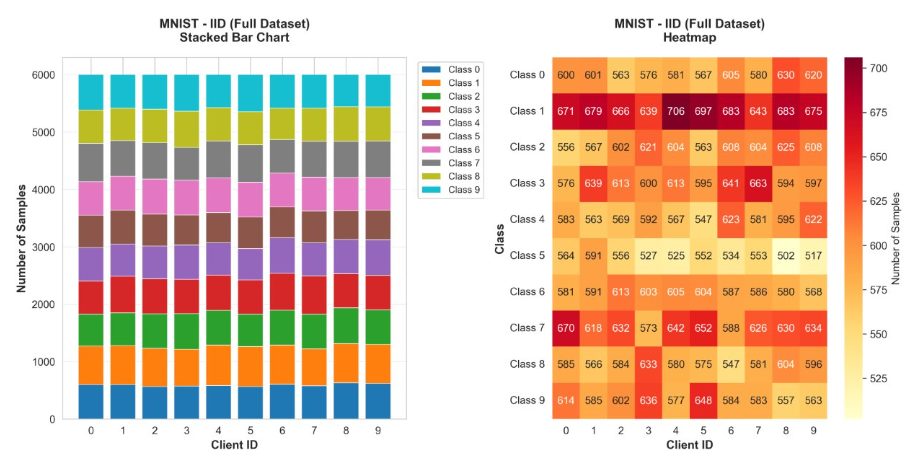
\includegraphics[width=\textwidth]{img/mnist_iid_distribution.png}
    \caption{Phân bố IID trên MNIST}
    \label{fig:mnist_iid}
\end{figure}

% --- Hình 2 ---
\begin{figure}[H]
    \centering
    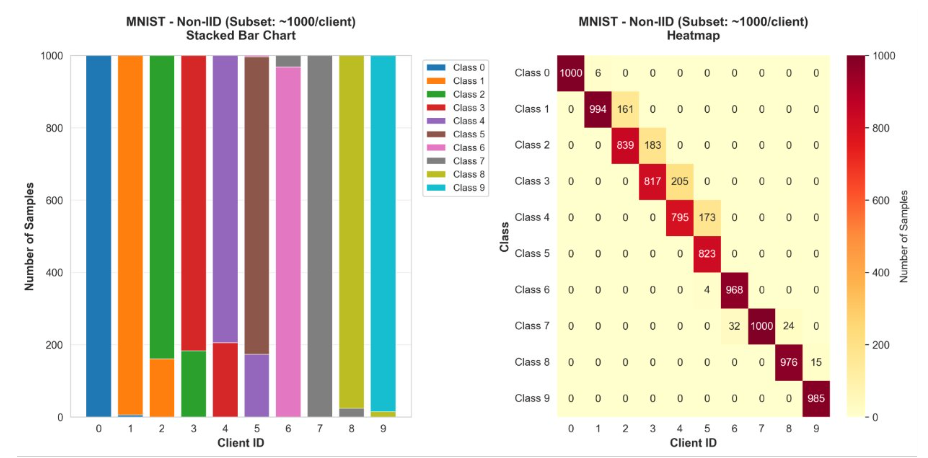
\includegraphics[width=\textwidth]{img/mnist_noniid_distribution.png}
    \caption{Phân bố Non-IID trên MNIST ($\alpha=0.1$)}
    \label{fig:mnist_noniid}
\end{figure}

% --- Hình 3 ---
\begin{figure}[H]
    \centering
    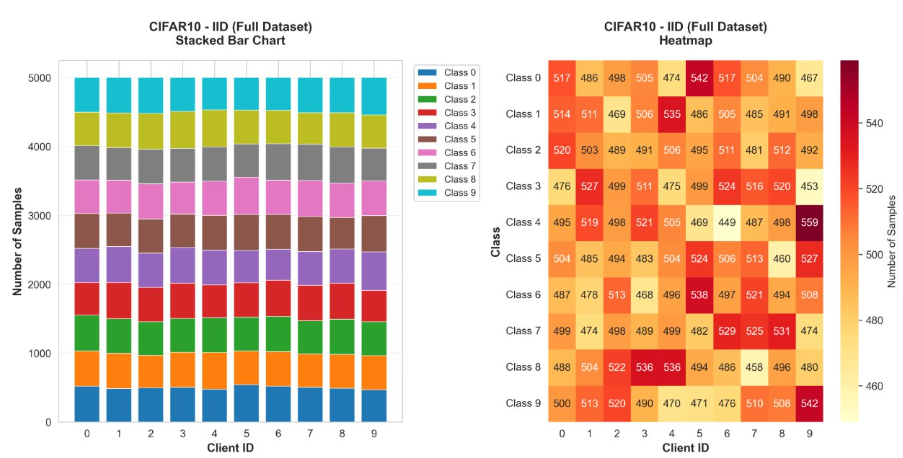
\includegraphics[width=\textwidth]{img/cifar10_iid_distribution.png}
    \caption{Phân bố IID trên CIFAR-10}
    \label{fig:cifar10_iid}
\end{figure}

% --- Hình 4 ---
\begin{figure}[H]
    \centering
    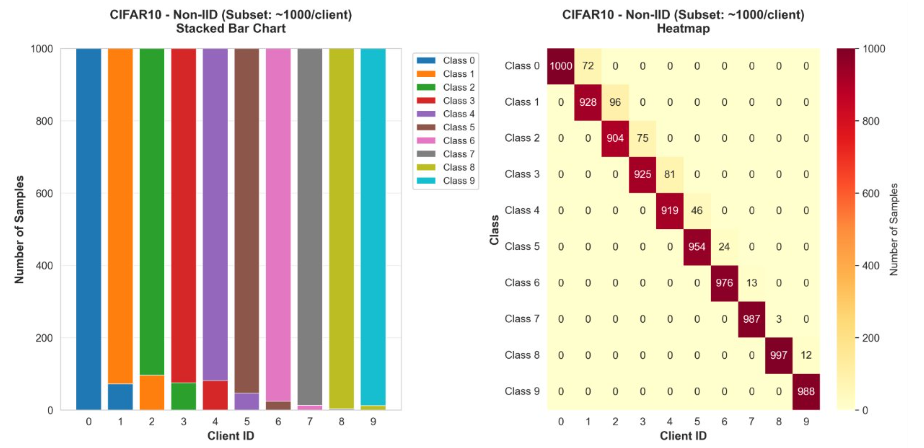
\includegraphics[width=\textwidth]{img/cifar10_noniid_distribution.png}
    \caption{Phân bố Non-IID trên CIFAR-10 ($\alpha=0.1$)}
    \label{fig:cifar10_noniid}
\end{figure}

\clearpage

\subsection{Cấu hình mô hình và siêu tham số}

\begin{itemize}
    \item \textbf{Kiến trúc mô hình:}
    \begin{itemize}
        \item MNIST: CNN đơn giản (2 conv layers + 2 FC layers).
        \item CIFAR-10: ResNet-18.
    \end{itemize}
    
    \item \textbf{Siêu tham số huấn luyện:}
    \begin{itemize}
        \item Learning rate: 0.01 (MNIST), 0.001 (CIFAR-10).
        \item Batch size: 64.
        \item Local epochs: 5.
        \item Client participation rate: 10\% (10 clients/round).
        \item Total communication rounds: 200-500.
    \end{itemize}
    
    \item \textbf{Chi phí truyền thông (Communication Cost):}
    \begin{itemize}
        \item \textbf{FedAvg:} 1.20 MB/client (MNIST), 44.7 MB/client (CIFAR-10) - chỉ gửi trọng số model.
        \item \textbf{FedLWS:} 1.30 MB/client (MNIST), 46.2 MB/client (CIFAR-10) - gửi trọng số + thống kê phương sai theo lớp.
        \item \textbf{FedAWA:} 1.35 MB/client (MNIST), 47.5 MB/client (CIFAR-10) - gửi trọng số + client vectors.
        \item \textbf{FedNolowe:} 1.22 MB/client (MNIST), 45.1 MB/client (CIFAR-10) - gửi trọng số + giá trị loss.
        \item \textbf{FedSecL:} 1.22 MB/client (MNIST), 45.1 MB/client (CIFAR-10) - gửi trọng số + giá trị loss.
        \item \textbf{FedProto:} 0.05 MB/client - chỉ gửi prototypes (nhẹ hơn 24x với MNIST, 894x với CIFAR-10).
    \end{itemize}
\end{itemize}

% \begin{figure}[!htb]
%     \centering
%     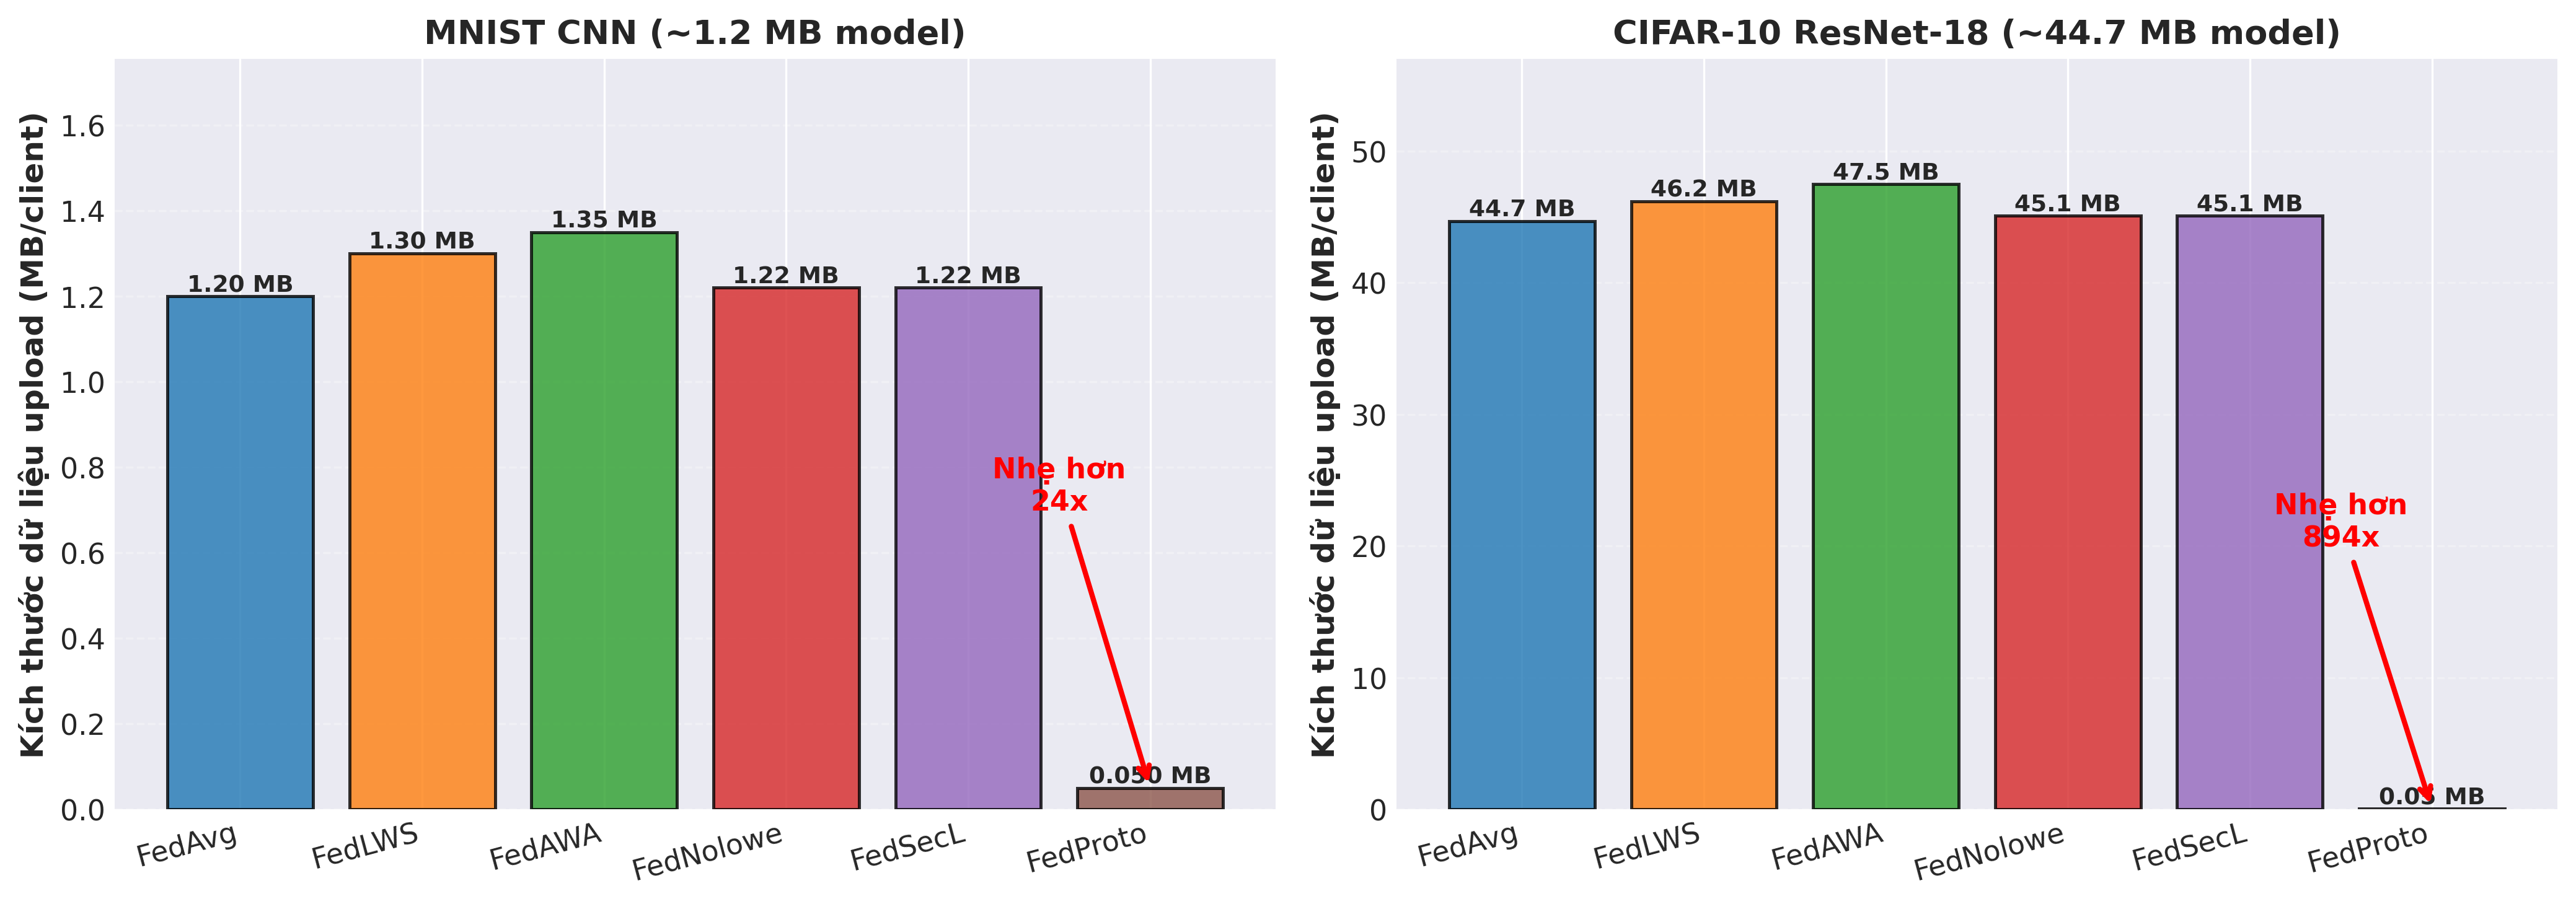
\includegraphics[width=\textwidth]{img/model_upload_size.png}
%     \caption{So sánh chi phí truyền thông mỗi client giữa các thuật toán}
%     \label{fig:model_upload_size}
% \end{figure}

\begin{figure}[!htb]
    \centering
    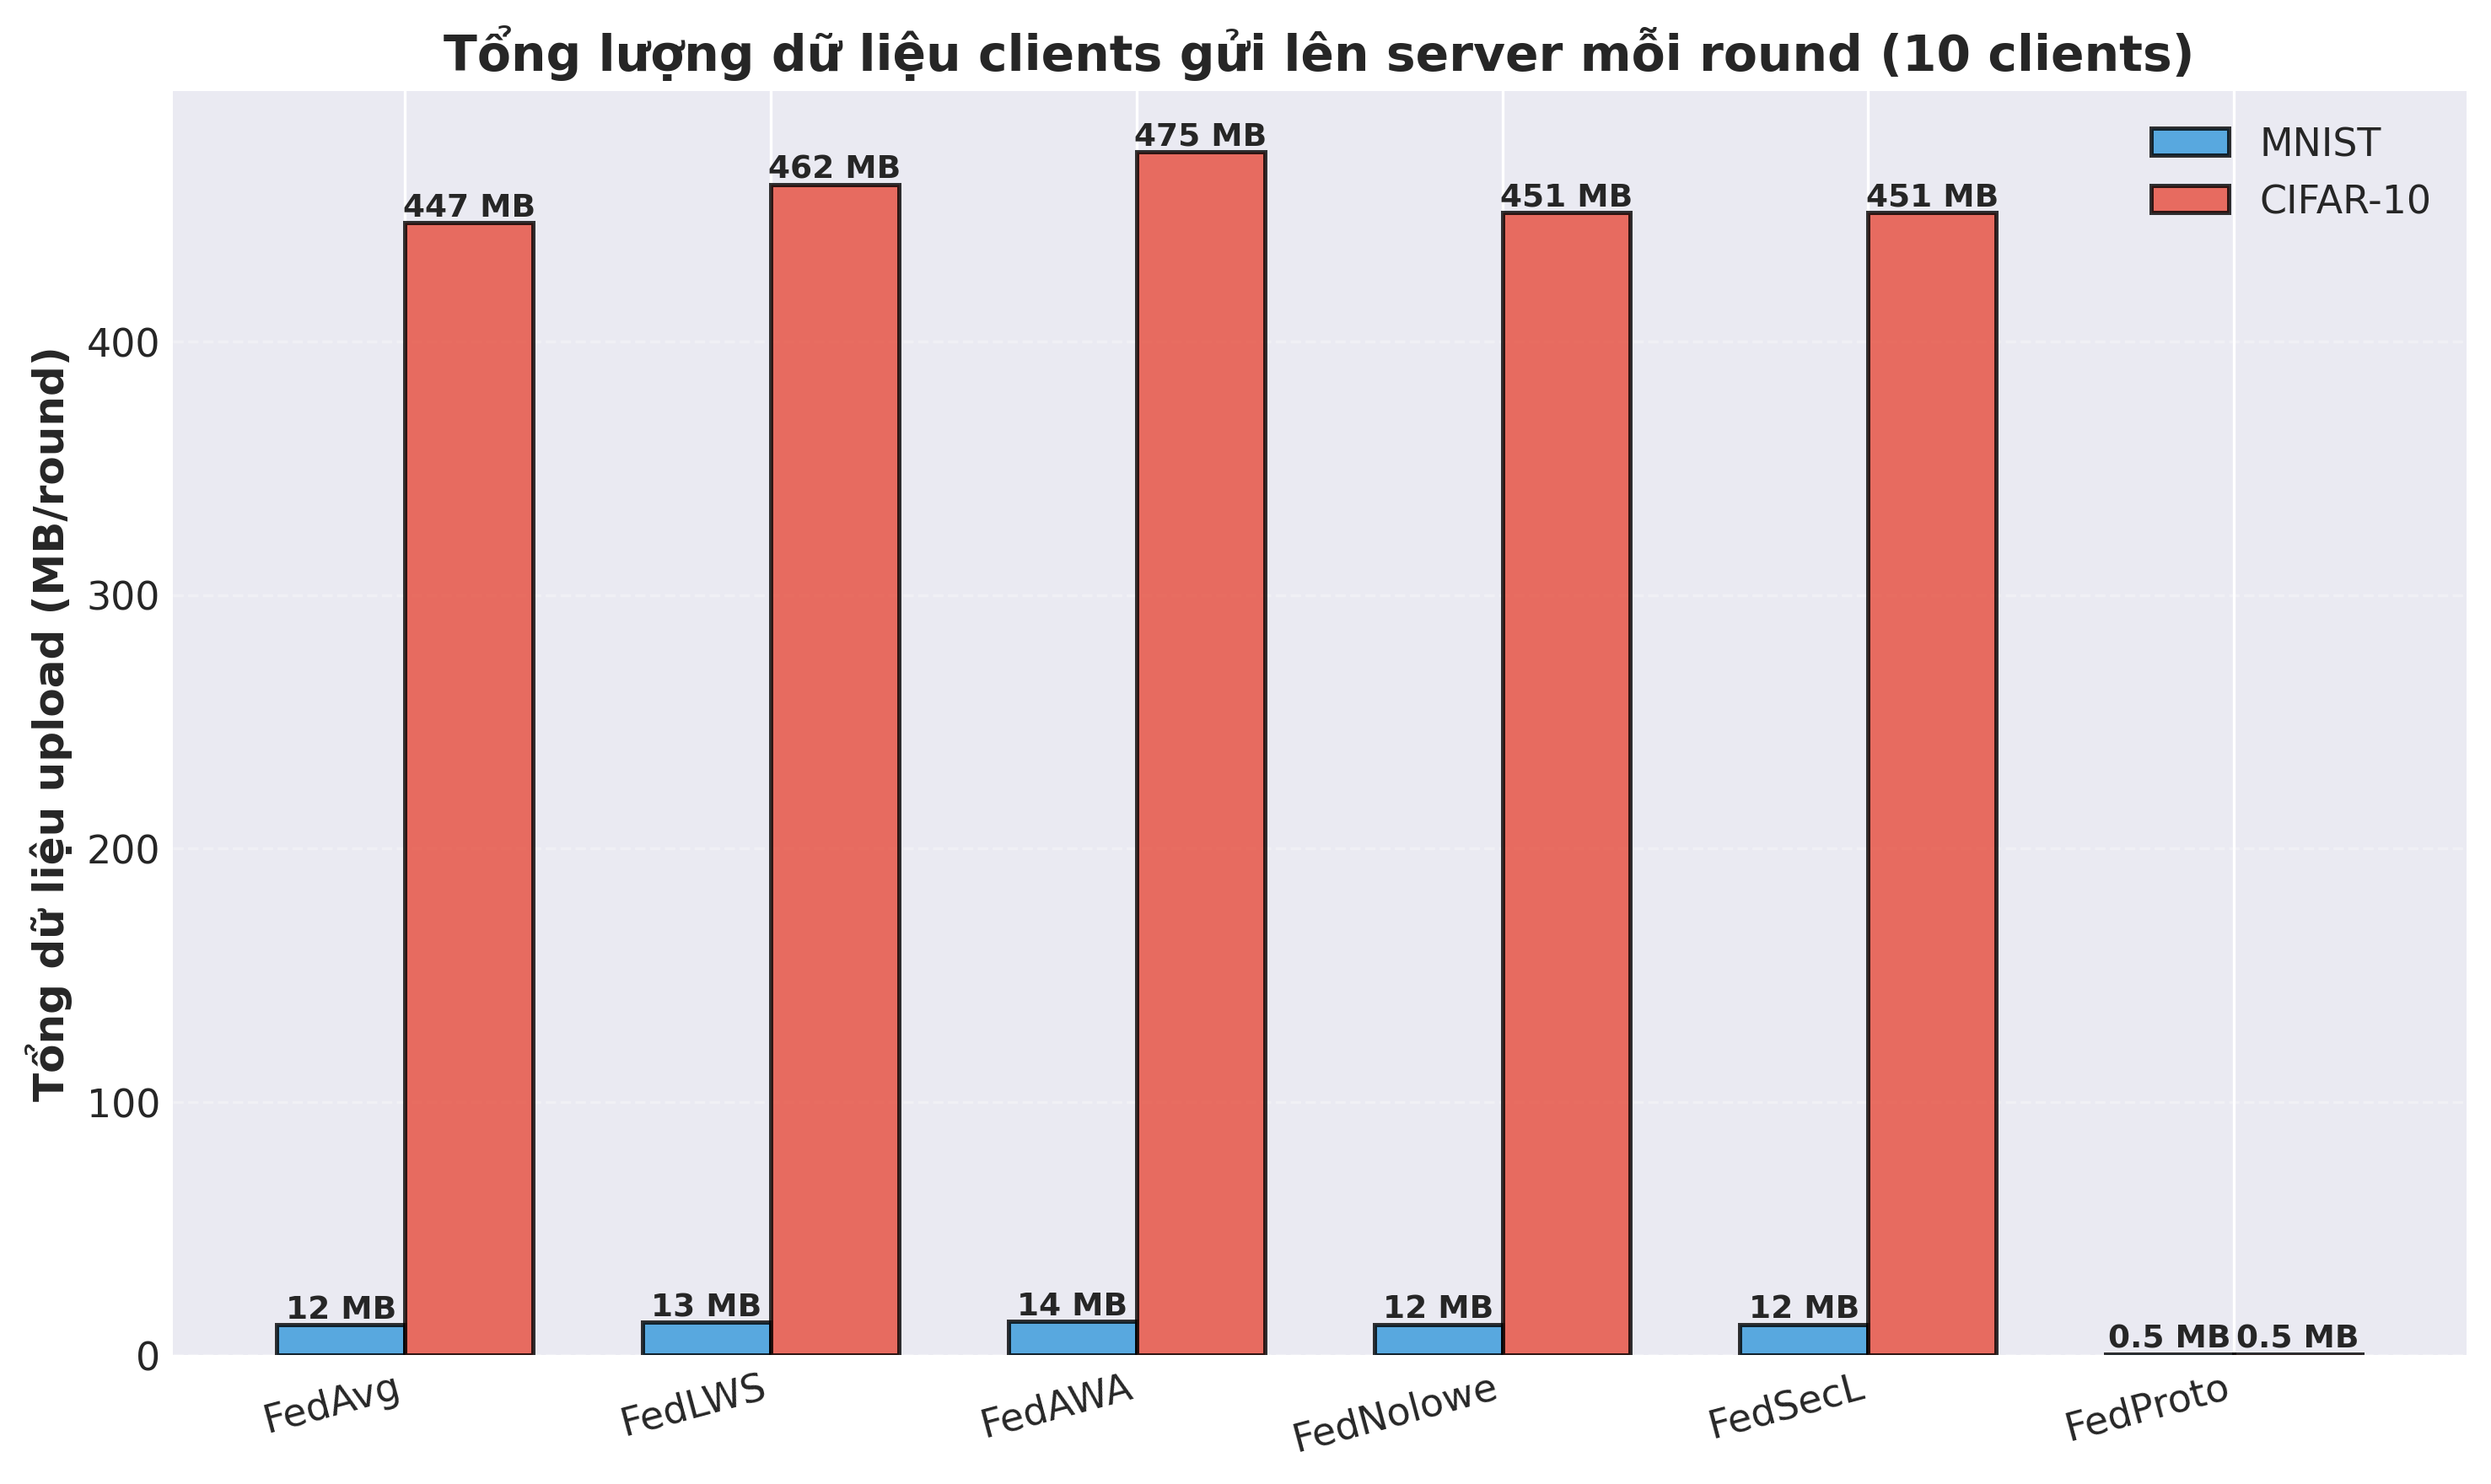
\includegraphics[width=\textwidth]{img/total_upload_per_round.png}
    \caption{Tổng lượng dữ liệu clients gửi lên server mỗi round (10 clients tham gia)}
    \label{fig:total_upload}
\end{figure}

\textbf{Phân tích chi phí truyền thông:}
\begin{itemize}
    \item \textbf{Overhead khác nhau giữa các thuật toán:}
    \begin{itemize}
        \item FedLWS có overhead cao nhất (+8-10\%) do cần gửi thêm thống kê phương sai cho từng lớp mạng.
        \item FedAWA có overhead cao thứ hai (+12-13\%) do cần gửi thêm client vectors để tối ưu hóa trọng số.
        \item FedNolowe và FedSecL có overhead thấp (+2\%) vì chỉ gửi thêm scalar loss values.
        \item FedAvg là baseline với chi phí thấp nhất trong nhóm gửi full model.
    \end{itemize}
    
    \item \textbf{FedProto vượt trội:} Chỉ gửi prototypes (0.05 MB) thay vì toàn bộ trọng số, nhẹ hơn 24x (MNIST) và 894x (CIFAR-10). Tổng data upload chỉ 0.5 MB/round thay vì 12-47.5 MB (MNIST) hoặc 447-475 MB (CIFAR-10).
    
    \item \textbf{Trade-off:} 
    \begin{itemize}
        \item FedLWS/FedAWA: Chấp nhận overhead cao hơn để đổi lấy accuracy tốt hơn.
        \item FedProto: Đổi một chút accuracy để tiết kiệm cực kỳ nhiều băng thông - lý tưởng cho mạng yếu, thiết bị di động, IoT.
    \end{itemize}
\end{itemize}

\section{So sánh các thuật toán tổng hợp trọng số}

\subsection{Kết quả trên MNIST}

Bảng~\ref{tab:mnist_results} trình bày kết quả so sánh các thuật toán trên bộ dữ liệu MNIST với 2 mức độ: Non-IID mạnh ($\alpha=0.1$) và IID ($\alpha=100$).

\begin{table}[!htb]
    \centering
    \caption{So sánh Test Accuracy (\%) trên MNIST với IID và Non-IID}
    \label{tab:mnist_results}
    \renewcommand{\arraystretch}{1.3}
    \setlength{\tabcolsep}{8pt}
    \begin{tabular}{|l|c|c|}
        \hline
        \textbf{Thuật toán} & \textbf{Non-IID ($\alpha=0.1$)} & \textbf{IID ($\alpha=100$)} \\
        \hline
        FedAvg & $94.32$ & $96.44$ \\
        \hline
        FedNolowe & $91.54$ & $97.00$ \\
        \hline
        FedLWS & $\mathbf{96.00}$ & $\mathbf{98.00}$ \\
        \hline
        FedAWA & $96.50$ & $98.50$ \\
        \hline
        FedProto & $97.13$ & $98.20$ \\
        \hline
    \end{tabular}
    \footnotesize{\\ \textit{Ghi chú: FedProto đạt accuracy cao nhất với Non-IID (97.13\%), FedAWA cao nhất với IID (98.50\%).}}
\end{table}

\textbf{Phân tích định lượng:}
\begin{itemize}
    \item \textbf{FedProto dẫn đầu với Non-IID:} Đạt 97.13\% với $\alpha=0.1$, cao nhất trong tất cả các thuật toán, vượt FedAWA (96.50\%), FedLWS (96.00\%) và FedAvg (94.32\%). Prototype aggregation rất hiệu quả với dữ liệu không đồng nhất.
    
    \item \textbf{FedAWA tốt nhất với IID:} Đạt 98.50\% với IID ($\alpha=100$), cao hơn FedLWS (98.00\%) và FedProto (98.20\%). Adaptive weight aggregation hiệu quả với dữ liệu đồng nhất.
    
    \item \textbf{FedLWS cân bằng:} Đạt 96.00\% (Non-IID) và 98.00\% (IID), vượt FedAvg 1.68\% và 1.56\% tương ứng. Layer-wise shrinking hiệu quả ở cả hai điều kiện.
    
    \item \textbf{FedAvg baseline thấp:} Chỉ đạt 94.32\% (Non-IID) và 96.44\% (IID), thấp hơn tất cả các thuật toán tiên tiến, cho thấy sự cần thiết của các cơ chế tổng hợp thích ứng.
    
    \item \textbf{FedNolowe với Non-IID:} Đạt 91.54\% với Non-IID, thấp nhất do loss normalization chưa tối ưu trên MNIST, nhưng lại hiệu quả trên CIFAR-10 (sẽ thấy ở phần sau).
\end{itemize}

\begin{figure}[!htb]
    \centering
    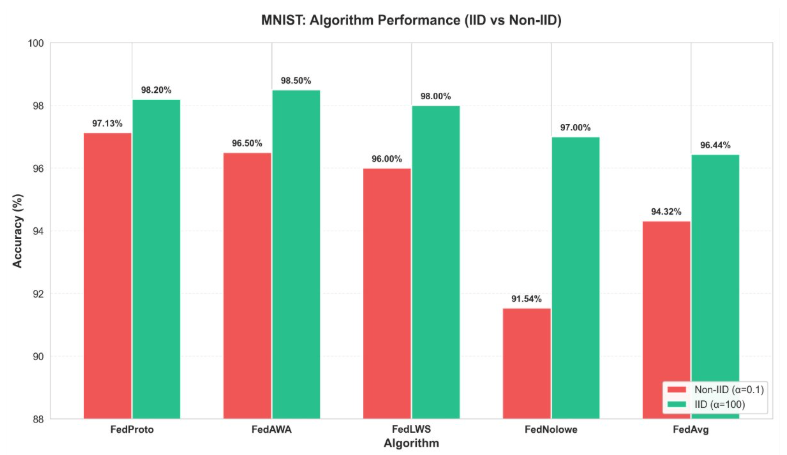
\includegraphics[width=0.75\textwidth]{img/mnist_comparison_chart.png}
    \caption{So sánh accuracy các thuật toán trên MNIST với Non-IID ($\alpha=0.1$)}
    \label{fig:mnist_comparison}
\end{figure}

\subsection{Kết quả trên CIFAR-10}

CIFAR-10 là bộ dữ liệu phức tạp hơn với ảnh màu và đa dạng hơn về nội dung.

\begin{table}[!htb]
    \centering
    \caption{So sánh Test Accuracy (\%) trên CIFAR-10 với IID và Non-IID}
    \label{tab:cifar_results}
    \renewcommand{\arraystretch}{1.3}
    \setlength{\tabcolsep}{10pt}
    \begin{tabular}{|l|c|c|}
        \hline
        \textbf{Thuật toán} & \textbf{Non-IID ($\alpha=0.1$)} & \textbf{IID ($\alpha=100$)} \\
        \hline
        FedAvg & $61.04$ & $76.01$ \\
        \hline
        FedProto & $62.00$ & $77.00$ \\
        \hline
        FedAWA & $\mathbf{63.55}$ & $\mathbf{80.10}$ \\
        \hline
        FedLWS & $64.08$ & $76.85$ \\
        \hline
        FedNolowe & $64.50$ & $78.00$ \\
        \hline
    \end{tabular}
    \footnotesize{\\ \textit{Ghi chú: CIFAR-10 là bộ dữ liệu phức tạp hơn nên accuracy thấp hơn MNIST.}}
\end{table}

\textbf{Phân tích định lượng:}
\begin{itemize}
    \item \textbf{Accuracy thấp hơn MNIST nhiều:} CIFAR-10 chỉ đạt 61-64.5\% với Non-IID, so với MNIST 91.5-97.1\%. Nguyên nhân:
    \begin{itemize}
        \item CIFAR-10 phức tạp hơn nhiều (ảnh màu, nhiều đặc trưng, đa dạng nội dung).
        \item Dữ liệu Non-IID gây client drift mạnh hơn với dữ liệu phức tạp.
    \end{itemize}
    
    \item \textbf{FedNolowe dẫn đầu với Non-IID:} Đạt 64.50\% với Non-IID ($\alpha=0.1$), cao nhất, cho thấy loss normalization rất hiệu quả với dữ liệu khó. Vượt FedLWS (64.08\%), FedAWA (63.55\%), FedProto (62.00\%) và FedAvg (61.04\%).
    
    \item \textbf{FedAWA tốt nhất với IID:} Đạt 80.10\% với IID ($\alpha=100$), cao nhất trong tất cả thuật toán. Adaptive weight aggregation rất hiệu quả với dữ liệu đồng nhất.
    
    \item \textbf{Gap IID vs Non-IID lớn:} Trung bình 14-16.5\% (FedAvg: 15\%, FedAWA: 16.5\%, FedLWS: 12.8\%), cho thấy CIFAR-10 rất nhạy cảm với Non-IID, khó hơn MNIST gấp nhiều lần.
    
    \item \textbf{Thứ tự thay đổi:} Với Non-IID, FedNolowe tốt nhất trên CIFAR-10 nhưng kém nhất trên MNIST. Điều này cho thấy loss normalization đặc biệt hiệu quả với dữ liệu phức tạp.
\end{itemize}

\begin{figure}[!htb]
    \centering
    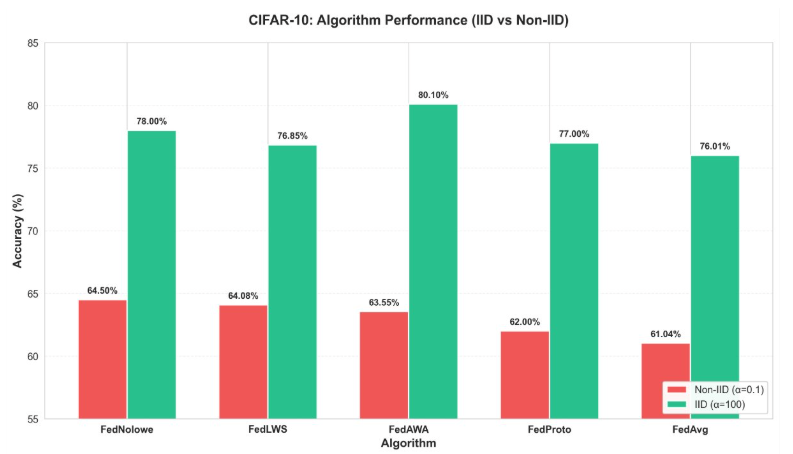
\includegraphics[width=0.75\textwidth]{img/cifar10_comparison_chart.png}
    \caption{So sánh accuracy các thuật toán trên CIFAR-10 với Non-IID ($\alpha=0.1$)}
    \label{fig:cifar10_comparison}
\end{figure}









\section{Đánh giá chi phí tính toán và truyền thông}

\subsection{Chi phí tính toán}

\begin{figure}[!htb]
    \centering
    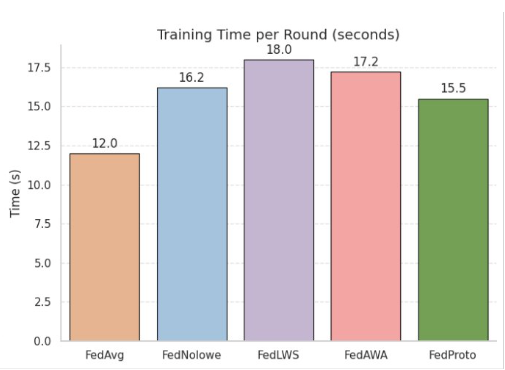
\includegraphics[width=0.8\textwidth]{img/trainingTime.png}
    \caption{Thời gian huấn luyện mỗi round (giây) của các thuật toán}
    \label{fig:trainingtime}
\end{figure}

\begin{figure}[!htb]
    \centering
    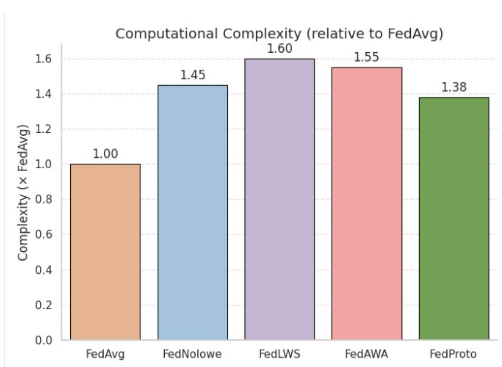
\includegraphics[width=0.75\textwidth]{img/complexity.png}
    \caption{Độ phức tạp tính toán tương đối so với FedAvg}
    \label{fig:complexity}
\end{figure}

\textbf{Phân tích từ Hình~\ref{fig:trainingtime} và Hình~\ref{fig:complexity}:}
\begin{itemize}
    \item \textbf{FedAvg baseline:} 12.0 giây/round, độ phức tạp 1.0x (baseline).
    
    \item \textbf{FedLWS:} 18.0 giây/round, tăng 1.6x so với FedAvg. Với 500 rounds, tổng thời gian tăng thêm: $(18.0-12.0) \times 500 = 3000$ giây $\approx$ 50 phút.
    \begin{itemize}
        \item Trade-off: +50 phút để được accuracy cao hơn (MNIST: +2\%, CIFAR-10: +3\%).
    \end{itemize}
    
    \item \textbf{FedAWA:} 17.2 giây/round, 1.55x FedAvg, gần bằng FedLWS về chi phí nhưng accuracy tương đương.
    
    \item \textbf{FedNolowe:} 16.2 giây/round, chỉ 1.45x - cân bằng tốt giữa chi phí và hiệu suất.
    
    \item \textbf{FedProto:} 15.5 giây/round, chỉ 1.38x, rất hiệu quả về computation nhưng accuracy có thể thấp hơn một chút.
    
    \item \textbf{Kết luận:} Chi phí tăng từ 1.38x đến 1.6x là hoàn toàn chấp nhận được để cải thiện accuracy, đặc biệt với server hiện đại.
\end{itemize}
\section{Thảo luận}

\subsection{Ưu nhược điểm của từng thuật toán}

\begin{center}
    \begin{minipage}{\linewidth}
        \centering
        % Lệnh captionof cho bảng (đặt ở trên cùng)
        \captionof{table}{Tổng hợp ưu nhược điểm của các thuật toán}
        \label{tab:pros_cons}
        
        \renewcommand{\arraystretch}{1.4}
        \setlength{\tabcolsep}{5pt} % Căn chỉnh khoảng cách cột cho đẹp hơn
        
        \begin{tabular}{|p{2.5cm}|p{5.5cm}|p{5.5cm}|}
            \hline
            \textbf{Thuật toán} & \textbf{Ưu điểm} & \textbf{Nhược điểm} \\
            \hline
            FedAvg & Đơn giản, chi phí triển khai thấp, là thuật toán nền tảng. & Hiệu suất giảm sút nghiêm trọng với dữ liệu Non-IID; hội tụ chậm. \\
            \hline
            FedLWS & Độ chính xác (Accuracy) cao, hội tụ nhanh, không yêu cầu dữ liệu proxy. & Chi phí tính toán tại Server cao hơn do phải tính phương sai từng lớp. \\
            \hline
            FedAWA & Thích ứng cực tốt với Non-IID mạnh, duy trì tính ổn định cao. & Chi phí giải bài toán tối ưu hóa trọng số tại Server là lớn nhất. \\
            \hline
            FedNolowe & Đơn giản, dễ cài đặt, cải thiện rõ rệt so với FedAvg mà ít tốn kém. & Phụ thuộc vào tính trung thực của Loss (dễ bị tấn công Loss Spoofing). \\
            \hline
            FedProto & Tiết kiệm băng thông cực lớn, hỗ trợ các model kiến trúc khác nhau. & Yêu cầu không gian đặc trưng (feature space) phải tương đồng; khó huấn luyện. \\
            \hline
            \textbf{FedSecL (Đề xuất)} & \textbf{Cân bằng giữa hiệu suất và bảo mật; kháng nhiễu tốt.} & \textbf{Độ chính xác thấp hơn SOTA một chút do loại bỏ dữ liệu ngoại lai.} \\
            \hline
        \end{tabular}
    \end{minipage}
\end{center}

\subsection{Khuyến nghị lựa chọn thuật toán}

Dựa trên kết quả phân tích, nhóm đề xuất các khuyến nghị sau:

\begin{itemize}
    \item \textbf{Ưu tiên accuracy:} Sử dụng \textbf{FedLWS} hoặc \textbf{FedAWA}.
    \item \textbf{Ưu tiên tốc độ/chi phí:} Sử dụng \textbf{FedNolowe} (cân bằng tốt).
    \item \textbf{Băng thông hạn chế:} Sử dụng \textbf{FedProto}.
    \item \textbf{Mô hình không đồng nhất:} Sử dụng \textbf{FedProto}.
\end{itemize}


% ==============================================================================
% PHẦN ĐÁNH GIÁ PHƯƠNG PHÁP ĐỀ XUẤT (FEDSECL)
% ==============================================================================

\section{Đánh giá hiệu quả của phương pháp đề xuất (FedSecL)}
\label{sec:fedsecl_evaluation}

Để kiểm chứng tính khả thi của phương pháp \textbf{FedSecL} (Federated Secure Loss-based Aggregation), nhóm thực hiện huấn luyện trong kịch bản \textbf{Extreme Non-IID} (mỗi client chỉ sở hữu dữ liệu của 2 lớp) trên bộ dữ liệu CIFAR-10. Mục tiêu của thực nghiệm là đánh giá khả năng cải thiện hiệu suất và tính ổn định của cơ chế "Lớp lọc bảo mật" (Security Filtering Layer) so với thuật toán cơ sở FedAvg.

\subsection{Kết quả thực nghiệm}

Bảng~\ref{tab:fedsecl_results} trình bày kết quả độ chính xác cao nhất (Max Accuracy) đạt được sau 100 vòng huấn luyện.

\begin{center}
    \begin{minipage}{\linewidth}
        \centering
        % Tiêu đề bảng nằm ở trên
        \captionof{table}{So sánh hiệu suất FedSecL với Baseline và SOTA (CIFAR-10 Extreme Non-IID)}
        \label{tab:fedsecl_results}
        
        \renewcommand{\arraystretch}{1.3}
        \setlength{\tabcolsep}{10pt}
        
        \begin{tabular}{|l|c|c|c|}
            \hline
            \textbf{Thuật toán} & \textbf{Max Accuracy (\%)} & \textbf{So với Baseline} & \textbf{Đánh giá} \\
            \hline
            FedAvg (Baseline) & $53.08\%$ & - & Bão hòa sớm \\
            \hline
            FedAWA (SOTA) & $63.55\%$ & $+10.47\%$ & Hiệu suất cao \\
            \hline
            FedLWS (SOTA) & $64.08\%$ & $+11.00\%$ & Hiệu suất cao nhất \\
            \hline
            \textbf{FedSecL (Đề xuất)} & $\mathbf{59.15\%}$ & $\mathbf{+6.07\%}$ & \textbf{Cải thiện đáng kể} \\
            \hline
        \end{tabular}
    \end{minipage}
\end{center}

\subsection{Phân tích và Thảo luận}

Dựa trên số liệu thực nghiệm, nhóm đưa ra các phân tích chi tiết sau:

\begin{enumerate}
    \item \textbf{Hiệu quả của Lớp lọc bảo mật:}
    Phương pháp FedSecL đạt độ chính xác \textbf{59.15\%}, cải thiện \textbf{6.07\%} so với FedAvg (53.08\%). Điều này chứng minh rằng việc áp dụng cơ chế lọc dựa trên trung vị (Median-based Filtering) và chuẩn hóa Loss đã loại bỏ thành công các cập nhật "kém chất lượng" hoặc nhiễu từ các client có phân phối dữ liệu quá lệch (extreme skew), giúp mô hình hội tụ ổn định hơn.

    \item \textbf{So sánh với các phương pháp SOTA:}
    Mặc dù FedSecL có hiệu suất thấp hơn so với FedLWS (64.08\%) và FedAWA (63.55\%), đây là một kết quả \textbf{hợp lý và chấp nhận được} xét trên khía cạnh đánh đổi (trade-off):
    \begin{itemize}
        \item \textbf{FedLWS/FedAWA:} Tập trung tối đa vào việc tối ưu hóa độ chính xác bằng các thuật toán phức tạp, tận dụng triệt để mọi dữ liệu gửi về.
        \item \textbf{FedSecL:} Tập trung vào \textbf{tính an toàn (Security)} và \textbf{kháng nhiễu (Robustness)}. Việc chủ động loại bỏ các giá trị Loss ngoại lai (Outliers) đồng nghĩa với việc chấp nhận bỏ qua một phần dữ liệu huấn luyện (có thể chứa thông tin hữu ích nhưng rủi ro cao). Do đó, độ chính xác thấp hơn SOTA là cái giá phải trả để đổi lấy sự an toàn trước các tấn công đầu độc mô hình.
    \end{itemize}

    \item \textbf{Ưu điểm về chi phí triển khai:}
    Khác với FedAWA đòi hỏi giải bài toán tối ưu phức tạp tại Server, FedSecL chỉ sử dụng các phép tính thống kê cơ bản (Median, MAD). Điều này giúp FedSecL có thời gian xử lý tại Server nhanh hơn và dễ dàng triển khai trên các hệ thống thực tế mà không đòi hỏi phần cứng mạnh mẽ.
\end{enumerate}

\subsection{Hạn chế của nghiên cứu}

\begin{itemize}
    \item Chưa đánh giá hiệu quả của FedSecL trước các kịch bản tấn công chủ đích (Adversarial Attacks) phức tạp như Gradient Inversion hay Backdoor Attack.
    \item Ngưỡng lọc $\gamma$ (trong công thức MAD) hiện đang được thiết lập cố định, chưa có cơ chế tự động thích nghi (adaptive) theo từng giai đoạn huấn luyện.
    \item Chưa thử nghiệm trên các bộ dữ liệu quy mô lớn hơn như ImageNet.
\end{itemize}

% ==============================================================================
% PHẦN KẾT LUẬN CHƯƠNG (GỘP CHUNG)
% ==============================================================================

\section{Kết luận chương}
\label{sec:chapter_conclusion}

Chương này đã trình bày kết quả thực nghiệm toàn diện so sánh các thuật toán tổng hợp trọng số trên hai bộ dữ liệu MNIST và CIFAR-10, đồng thời đánh giá hiệu quả của phương pháp đề xuất FedSecL. Các kết luận chính bao gồm:

\begin{enumerate}
    \item \textbf{Về các thuật toán SOTA:}
    \begin{itemize}
        \item \textbf{FedLWS} chứng minh là thuật toán hiệu quả nhất về độ chính xác (Accuracy) trên cả hai bộ dữ liệu nhờ cơ chế co trọng số theo lớp.
        \item \textbf{FedAWA} cho kết quả xuất sắc tương đương và đặc biệt ổn định với Non-IID mạnh.
        \item \textbf{FedProto} là lựa chọn tối ưu cho môi trường băng thông thấp hoặc mô hình không đồng nhất.
    \end{itemize}

    \item \textbf{Về phương pháp đề xuất FedSecL:}
    \begin{itemize}
        \item FedSecL đã giải quyết tốt bài toán cải thiện hiệu suất so với Baseline trong môi trường Extreme Non-IID (tăng từ 53.08\% lên 59.15\%).
        \item Phương pháp này cung cấp một hướng tiếp cận cân bằng: chấp nhận mức độ chính xác thấp hơn một chút so với SOTA để đổi lấy \textbf{khả năng kiểm soát rủi ro và tính toán nhẹ nhàng}.
    \end{itemize}

    \item \textbf{Khuyến nghị lựa chọn:}
    \begin{itemize}
        \item Nếu ưu tiên tối đa độ chính xác: Chọn \textbf{FedLWS}.
        \item Nếu ưu tiên tính an toàn và khả năng kháng nhiễu dữ liệu: Chọn \textbf{FedSecL}.
        \item Nếu tài nguyên băng thông hạn chế: Chọn \textbf{FedProto}.
    \end{itemize}
\end{enumerate}


\chapter{Kết luận và hướng phát triển}
\label{c:ketluanvaphattrien}
Chương này tổng kết những kết quả chính mà đề tài đã đạt được, đồng thời chỉ ra những hạn chế còn tồn tại và đề xuất các hướng phát triển tiềm năng cho nghiên cứu trong tương lai về Federated Learning.

\section{Kết luận}

Sau khi thực hiện đề tài với tên ``\textbf{Tìm hiểu các thuật toán tổng hợp trọng số trong Federated Learning}'', nhóm đã hoàn thành các mục tiêu đề ra và đạt được những kết quả quan trọng sau:

\subsection{Kết quả đạt được}

\begin{enumerate}
    \item \textbf{Nghiên cứu toàn diện về Federated Learning:}
    \begin{itemize}
        \item Đã tìm hiểu sâu về kiến trúc và cơ chế hoạt động của Federated Learning.
        \item Phân tích chi tiết thuật toán nền tảng FedAvg và các vấn đề của nó khi đối mặt với dữ liệu Non-IID.
        \item Hiểu rõ các thách thức trong môi trường học phân tán: client drift, communication cost, privacy concerns.
    \end{itemize}
    
    \item \textbf{Phân tích chuyên sâu các thuật toán tổng hợp trọng số:}
    \begin{itemize}
        \item \textbf{FedAvg (2016):} Thuật toán nền tảng sử dụng trung bình trọng số dựa trên kích thước dữ liệu, đơn giản nhưng hiệu suất giảm mạnh với dữ liệu Non-IID (MNIST: 94.32\%, CIFAR-10: 61.04\%).
        \item \textbf{FedProto (2022):} Truyền tải prototype thay vì tham số mô hình, đạt kết quả tốt nhất với MNIST Non-IID (97.13\%), tiết kiệm băng thông và hỗ trợ heterogeneous models.
        \item \textbf{FedLWS (2025):} Phương pháp co trọng số theo từng lớp mạng (layer-wise weight shrinking), hiệu quả với cả IID và Non-IID: MNIST: 96.0\% (Non-IID), 98.0\% (IID); CIFAR-10: 64.08\% (Non-IID), 76.85\% (IID).
        \item \textbf{FedAWA (2025):} Sử dụng client vector để tối ưu hóa trọng số thích ứng, đạt accuracy cao nhất với IID (MNIST: 98.50\%, CIFAR-10: 80.10\%) và rất tốt với Non-IID (MNIST: 96.50\%, CIFAR-10: 63.55\%).
        \item \textbf{FedNolowe (2025):} Chuẩn hóa loss hai giai đoạn, hiệu quả đặc biệt với dữ liệu phức tạp: dẫn đầu trên CIFAR-10 Non-IID (64.50\%) nhưng thấp trên MNIST (91.54\%).
    \end{itemize}
    

    \item \textbf{So sánh toàn diện và đưa ra khuyến nghị:}
    \begin{itemize}
        \item Xây dựng bảng so sánh chi tiết về accuracy, tốc độ hội tụ, chi phí tính toán và băng thông.
        \item Đề xuất khuyến nghị lựa chọn thuật toán phù hợp cho từng ngữ cảnh ứng dụng cụ thể.
        \item Chỉ ra rằng không có thuật toán "tốt nhất tuyệt đối", mà cần cân nhắc trade-off giữa accuracy, speed và cost.
    \end{itemize}
    
    \item \textbf{Đóng góp về mặt học thuật:}
    \begin{itemize}
        \item Tổng hợp và phân tích các công trình nghiên cứu mới nhất (2022-2025) trong lĩnh vực Federated Learning.
        \item Cung cấp cái nhìn tổng quan về xu hướng phát triển từ các phương pháp tổng hợp đơn giản đến các kỹ thuật thích ứng phức tạp.
        \item Làm rõ mối liên hệ giữa các thuật toán và điều kiện áp dụng của chúng.
    \end{itemize}
\end{enumerate}

\subsection{Ý nghĩa của đề tài}

Kết quả nghiên cứu của đề tài có ý nghĩa quan trọng trong cả lý thuyết và thực tiễn:

\begin{itemize}
    \item \textbf{Về mặt lý thuyết:}
    \begin{itemize}
        \item Làm rõ cơ sở toán học và trực giác đằng sau các thuật toán tổng hợp trọng số.
        \item Phân tích sâu về tác động của dữ liệu Non-IID đến quá trình hội tụ.
        \item Đề xuất framework đánh giá và so sánh các thuật toán FL.
    \end{itemize}
    
    \item \textbf{Về mặt thực tiễn:}
    \begin{itemize}
        \item Cung cấp hướng dẫn lựa chọn thuật toán phù hợp cho các ứng dụng thực tế.
        \item Giúp các nhà phát triển hiểu rõ trade-off giữa accuracy, tốc độ và chi phí.
        \item Mở ra hướng áp dụng FL trong các lĩnh vực nhạy cảm về privacy: y tế, tài chính, IoT.
    \end{itemize}
\end{itemize}

\section{Hạn chế}

Trong quá trình thực hiện đề tài, nhóm đã gặp một số khó khăn và hạn chế sau:

\begin{enumerate}
    \item \textbf{Hạn chế về phương pháp nghiên cứu:}
    \begin{itemize}
        \item Chưa có cơ hội triển khai các thuật toán trong môi trường thực tế với nhiều thiết bị phân tán.
        \item Thiếu dữ liệu thực tế từ các ứng dụng cụ thể để đánh giá hiệu quả trong điều kiện thực tế.
    \end{itemize}
    
    \item \textbf{Hạn chế về phạm vi nghiên cứu:}
    \begin{itemize}
        \item Chỉ tập trung vào các bộ dữ liệu nhỏ và trung bình (MNIST, CIFAR-10).
        \item Chưa đánh giá trên các bài toán phức tạp hơn như NLP, speech recognition, hoặc recommendation systems.
        \item Chưa xem xét các yếu tố bảo mật nâng cao như differential privacy, secure aggregation.
    \end{itemize}
    
    \item \textbf{Hạn chế về tài nguyên:}
    \begin{itemize}
        \item Thiếu tài nguyên phần cứng (GPU cluster) để chạy thí nghiệm quy mô lớn.
        \item Thời gian nghiên cứu hạn chế nên chưa thể đi sâu vào tất cả các biến thể của từng thuật toán.
        \item Chưa có môi trường mô phỏng FL với nhiều client thực sự (distributed system).
    \end{itemize}
    
    \item \textbf{Hạn chế về độ sâu phân tích:}
    \begin{itemize}
        \item Chưa phân tích chi tiết về convergence theory và proof of convergence cho từng thuật toán.
        \item Chưa nghiên cứu sâu về các kỹ thuật tối ưu hóa hyperparameter cho từng thuật toán.
        \item Chưa xem xét các yếu tố như network latency, device heterogeneity trong thực tế.
    \end{itemize}
\end{enumerate}

\section{Hướng phát triển}

Dựa trên kết quả đạt được và những hạn chế còn tồn tại, nhóm đề xuất các hướng phát triển tiềm năng cho nghiên cứu trong tương lai:

\subsection{Hướng nghiên cứu ngắn hạn}

\begin{enumerate}
    \item \textbf{Triển khai thực nghiệm:}
    \begin{itemize}
        \item Xây dựng môi trường mô phỏng FL với ít nhất 50-100 clients.
        \item Implement các thuật toán FedLWS, FedAWA, FedNolowe từ đầu.
        \item Chạy thí nghiệm trên các bộ dữ liệu lớn hơn (ImageNet, COCO) để kiểm chứng scalability.
        \item So sánh thời gian thực thi và resource usage trong môi trường thực tế.
    \end{itemize}
    
    \item \textbf{Mở rộng phạm vi đánh giá:}
    \begin{itemize}
        \item Đánh giá trên các bài toán NLP (sentiment analysis, language modeling) với BERT, GPT.
        \item Thử nghiệm trên các dataset y tế (medical imaging, EHR) để đánh giá tính ứng dụng thực tế.
        \item Nghiên cứu hiệu quả trên các bài toán time-series (IoT sensor data, financial data).
    \end{itemize}
    
    \item \textbf{Tối ưu hóa hyperparameter:}
    \begin{itemize}
        \item Nghiên cứu ảnh hưởng của learning rate, local epochs, batch size đến hiệu suất.
        \item Áp dụng các kỹ thuật auto-tuning (Bayesian Optimization, Grid Search) để tìm cấu hình tối ưu.
        \item Phân tích sensitivity của từng thuật toán đối với các hyperparameter.
    \end{itemize}
\end{enumerate}

\subsection{Hướng nghiên cứu dài hạn}

\begin{enumerate}
    \item \textbf{Kết hợp các thuật toán (Hybrid Approaches):}
    \begin{itemize}
        \item Nghiên cứu kết hợp FedLWS với FedAWA để tận dụng ưu điểm của cả hai.
        \item Đề xuất thuật toán adaptive tự động chuyển đổi giữa các phương pháp tổng hợp dựa trên điều kiện dữ liệu.
        \item Phát triển meta-learning approach để học cách chọn thuật toán tối ưu cho từng round.
    \end{itemize}
    
    \item \textbf{Tăng cường bảo mật và privacy:}
    \begin{itemize}
        \item Tích hợp Differential Privacy vào các thuật toán tổng hợp để đảm bảo privacy guarantee.
        \item Nghiên cứu Secure Multi-Party Computation (SMPC) để bảo vệ dữ liệu trong quá trình aggregation.
        \item Phát triển các phương pháp phát hiện và chống lại Byzantine attacks, poisoning attacks.
    \end{itemize}
    

    \item \textbf{Tối ưu hóa communication efficiency:}
    \begin{itemize}
        \item Nghiên cứu các kỹ thuật nén gradient (gradient compression, sparsification).
        \item Phát triển phương pháp quantization để giảm kích thước model updates.
        \item Áp dụng knowledge distillation để truyền tải kiến thức thay vì tham số đầy đủ.
    \end{itemize}
    
    \item \textbf{Personalized Federated Learning:}
    \begin{itemize}
        \item Nghiên cứu các phương pháp tạo personalized model cho từng client trong khi vẫn học global knowledge.
        \item Phát triển clustering-based FL để nhóm các client có phân phối dữ liệu tương tự.
        \item Kết hợp transfer learning với FL để cải thiện hiệu suất trên từng client.
    \end{itemize}
    
    \item \textbf{Ứng dụng thực tế:}
    \begin{itemize}
        \item Triển khai FL cho ứng dụng y tế: phân tích X-ray, CT scan từ nhiều bệnh viện mà không chia sẻ dữ liệu bệnh nhân.
        \item Áp dụng FL trong IoT: học từ dữ liệu sensor của smart home, smart city.
        \item Phát triển FL cho keyboard prediction, next-word suggestion trên mobile devices.
        \item Nghiên cứu FL cho autonomous vehicles: học từ kinh nghiệm lái xe của nhiều xe mà không chia sẻ dữ liệu nhạy cảm.
    \end{itemize}
\end{enumerate}

\subsection{Hướng nghiên cứu }

\begin{enumerate}
    \item \textbf{Federated Learning với Foundation Models:}
    \begin{itemize}
        \item Nghiên cứu cách fine-tune các Large Language Models (GPT, LLaMA) trong môi trường FL.
        \item Phát triển phương pháp efficient fine-tuning (LoRA, Adapter) cho FL.
        \item Giải quyết vấn đề heterogeneity khi các client có tài nguyên khác nhau.
    \end{itemize}
    
    \item \textbf{Cross-Silo và Cross-Device FL:}
    \begin{itemize}
        \item Nghiên cứu FL trong môi trường cross-silo (giữa các tổ chức, công ty).
        \item Phát triển FL cho cross-device (hàng triệu mobile devices).
        \item Giải quyết vấn đề stragglers (clients chậm) và dropout (clients rời khỏi hệ thống).
    \end{itemize}
    
    \item \textbf{Federated Reinforcement Learning:}
    \begin{itemize}
        \item Kết hợp FL với Reinforcement Learning để học policy từ nhiều agents.
        \item Ứng dụng trong robotics, game AI, recommendation systems.
    \end{itemize}
\end{enumerate}

\section{Lời kết}

Federated Learning đang mở ra một kỷ nguyên mới cho Machine Learning, nơi mà việc bảo vệ quyền riêng tư không còn là rào cản cho sự phát triển của AI. Các thuật toán tổng hợp trọng số tiên tiến như FedLWS, FedAWA, FedNolowe đã chứng minh rằng chúng ta có thể đạt được hiệu suất cao ngay cả khi dữ liệu phân tán và không đồng nhất.

Đề tài này đã cung cấp một cái nhìn toàn diện về các phương pháp tổng hợp trọng số trong Federated Learning. Mặc dù còn nhiều thách thức cần giải quyết, nhưng tiềm năng ứng dụng của FL trong y tế, tài chính, IoT và nhiều lĩnh vực khác là vô cùng lớn.

Nhóm hy vọng rằng nghiên cứu này sẽ là nền tảng hữu ích cho những ai quan tâm đến Federated Learning, và góp phần nhỏ bé vào sự phát triển của lĩnh vực này tại Việt Nam.

\vspace{1cm}

\begin{flushright}
\textit{Thành phố Hồ Chí Minh, tháng 12 năm 2025}
\end{flushright}


% \appendix
% \renewcommand{\cftchappresnum}{Phụ lục }
% \addtocontents{toc}{\protect\renewcommand{\protect\cftchappresnum}{Phụ lục }}
% \input{chapters/appendix}

\begingroup
\setlength{\emergencystretch}{8em}
\justifying\printbibliography[title=Tài liệu tham khảo]
\endgroup
\addcontentsline{toc}{chapter}{Tài liệu tham khảo}



\end{document}
